\chapter{因果响应}
\label{chap:causal-inference}

接受培训的人平均成绩更高，是培训提高了成绩，还是基础较好的人更愿意参加培训？
第~\ref{chap:random-variables}章已经建立条件分布与统计推断，第
~\ref{chap:information-theory-and-statistical-geometry}章进一步比较分布及其对任务的
影响。但把成绩预测得很准，仍不能回答主动安排培训以后会发生什么。后一个问题要求
说明：改变的究竟是对已有记录的筛选，还是产生记录的机制。

本章研究因果响应及生成它的结构。响应把行动与个体背景映射为结果；生成结构进一步
说明这个整体映射由哪些局部关系和机制合成。我们以处理\(T\)、结果\(Y\)与处理前
信息\(X\)为共同例子，区分给定模型的计算、数据对响应的识别，以及数据对生成结构的
推断。模型明确给定时，可以直接比较行动，也可以在得知某人的事实以后计算替代结果；
这不意味着数据已经证明该模型正确。反过来，有些平均响应可以由实验设计识别，而无须
唯一恢复每一个局部方程。

阅读上先把响应当作可使用的数学对象，明确输入、行动规则和背景分布，再分别比较个体、
总体及局部变化。事实证据只更新对背景的认识，替代行动则改变响应映射。识别部分检查
数据能否支持这些答案，结构部分才打开模型内部，证明无环局部机制怎样实现前面使用的
映射，并建立本章所需的图语义。这样可以始终区分“在模型内算得出”与“由资料确定得了”。

\section{因果响应的表示}
\label{sec:causal-response-representation}

要询问一个人接受培训后的成绩，至少需要说明培训方案、这个人的背景、成绩测量时间，
以及安排培训会改变哪些生成规则。只给出一个拟合函数
\(\mathbb E[Y\mid T=t,X=x]\)还不够：它描述自然分配下的条件平均，未必描述主动安排
培训的后果。本节先规定能够回答行动问题的最低模型接口，暂不要求把全部内部结构画成图。

\subsection{原因与背景的响应表示}
\label{sec:causal-observation-generation}

用\(t\)表示可以设定的处理值，用\(\bm u\)表示在所比较行动之间保持的个体背景。
背景包含模型没有继续解释的差异，例如既有能力和未测量的环境因素；它与“所有已观测
协变量”不是同义词。模型\(M\)规定背景的联合分布、自然运行规则和允许的行动。
本节假定这些规则已经给出唯一结果，后面再说明怎样从局部方程保证这一点。

\begin{definition}[因果响应与自然、行动映射]
  \label{def:causal-response-interface}
  给定背景可测空间\((\mathcal U,\mathscr U)\)及概率测度\(P_{\bm U}\)，
  自然变量的可测状态空间\(\mathcal V\)，处理空间\(\mathcal T\)和结果空间
  \(\mathcal Y\)。固定模型\(M\)提供唯一值的可测自然映射
  \(F_M:\mathcal U\to\mathcal V\)，以及每个允许行动\(a\)的唯一值可测映射
  \(F_M^a:\mathcal U\to\mathcal V\)。后者由模型指定的机制替换产生，而非任意另选函数。
  若\(a(t)\)表示把处理设为\(t\)的允许行动，\(\pi_Y\)表示取结果坐标，则
  \term{因果响应}（causal response）是映射
  \begin{equation}
    R_M:\mathcal T\times\mathcal U\longrightarrow\mathcal Y,
    \qquad
    R_M(t,\bm u)=\pi_Y\bigl(F_M^{a(t)}(\bm u)\bigr).
    \label{eq:causal-response-interface}
  \end{equation}
  本章要求\(R_M\)对乘积可测结构可测。自然变量为
  \(\bm V=F_M(\bm U)\)，行动后的变量为\(\bm V_a=F_M^a(\bm U)\)。
\end{definition}

固定\(\bm u\)时，\(t\mapsto R_M(t,\bm u)\)回答同一单位怎样响应不同处理；
让\(\bm U\)按\(P_{\bm U}\)变化，才得到总体响应分布。外生背景的各分量可以相关，
定义没有默许独立性。若采用有限维参数表示\(M_{\bm\theta}\)，参数
\(\bm\theta\)描述研究者选定的机制；修改拟合参数是在改变模型，设置\(t\)则是在一个
固定模型内行动。两种变化不能互相代替。

下面用两套二元机制计算这一区别。设背景满足
\[
  U\sim\operatorname{Bernoulli}(1/2).
\]
处理与结果均取\(0,1\)。模型甲为
\begin{equation}
  T=U,\qquad Y=U;
  \label{eq:causal-observational-equivalence-confounding}
\end{equation}
模型乙为
\begin{equation}
  T=U,\qquad Y=T.
  \label{eq:causal-observational-equivalence-effect}
\end{equation}
两者自然映射都是\(F_M(u)=(u,u)\)，从而
\[
  \begin{aligned}
    \mathbb P(T=0,Y=0)&=\mathbb P(T=1,Y=1)=\frac12,\\
    \mathbb P(T=0,Y=1)&=\mathbb P(T=1,Y=0)=0.
  \end{aligned}
\]
在甲中，处理不进入结果规则；在乙中，结果直接复制处理。若允许的行动是把处理规则
替换为常数\(t\)，保留结果规则，则
\[
  F_{M_{\text{甲}}}^{a(t)}(u)=(t,u),\qquad
  F_{M_{\text{乙}}}^{a(t)}(u)=(t,t),
\]
所以\(R_{M_{\text{甲}}}(t,u)=u\)，而
\(R_{M_{\text{乙}}}(t,u)=t\)。两模型的自然映射相同，行动映射不同；
观测记录无法仅凭样本量区分这种差异。

\subsection{机制干预下的潜在结果}
\label{sec:causal-intervention-potential-outcomes}

上例没有筛出自然接受处理的人，而是改变了处理怎样产生。这就是机制干预：
指定一项生成规则的替换，再让其余规则根据新的输入继续运行。行动的因果含义来自
这种替换约定，不来自函数名称或概率记号。

\begin{definition}[理想干预]
  \label{def:causal-intervention}
  对给定模型的处理变量\(T\)作\term{干预}（intervention）
  \(\operatorname{do}(T=t)\)，表示删除自然生成\(T\)的规则，并以常量规则
  \(T=t\)替换。其余生成规则和指定的背景分布\(P_{\bm U}\)保持不变。
  由行动映射\(F_M^{a(t)}\)推前得到的分布记作
  \(P^{\operatorname{do}(T=t)}\)。
\end{definition}

“其余规则不变”不是说其余变量的取值不变。若培训改变技能，技能再影响成绩，
行动后技能和成绩都应重算。只锁住所有非处理字段再评估一个预测器，通常不是这一行动。
多变量行动同样由\(F_M^a\)表达，但模型必须说明哪些规则替换、哪些保留。

\begin{definition}[潜在结果]
  \label{def:causal-potential-outcomes}
  对明确的目标总体、处理版本和结果测量时间，\term{潜在结果}
  （potential outcome）是随机变量
  \begin{equation}
    Y(t)=R_M(t,\bm U).
    \label{eq:causal-response-potential-outcome}
  \end{equation}
  对二元处理，\((Y(0),Y(1))\)定义在同一背景概率空间上；两项分别表示同一单位
  在两种处理下的结果，而不是分别抽取两个人。
\end{definition}

可测性保证可以讨论潜在结果的概率规律。记\(\mathcal L(Z)\)为随机变量\(Z\)的分布，
则
\[
  \mathcal L(Y(t))
  =
  (R_M(t,\cdot))_{\#}P_{\bm U}
  =
  \mathcal L(Y\mid\operatorname{do}(T=t)).
\]
符号\(\#\)表示第~\ref{sec:rv-pushforward}节的分布推前。这里的
\(\operatorname{do}\)标记修改后的模型，不是对自然事件\(T=t\)作普通条件化。
潜在结果聚焦所选行动下的输出；仅有一张潜在结果表，并不自动给出其他变量的完整
生成机制\scite{math-hernan2020whatif}

观察条件分布\(p(y\mid T=t)\)会筛选自然规则恰好给出处理\(t\)的单位，因而同时
包含处理作用和进入处理组的选择。在上面两套机制中，都有
\[
  \mathbb P(Y=1\mid T=1)=1,\qquad
  \mathbb P(Y=1\mid T=0)=0.
\]
但对甲，设定处理以后结果仍为\(U\)，故
\[
  \mathbb P(Y=1\mid\operatorname{do}(T=t))=\frac12,
  \qquad t\in\{0,1\};
\]
对乙，设定处理以后结果为\(t\)，故
\[
  \mathbb P(Y=1\mid\operatorname{do}(T=t))=t.
\]
相同的观测关联对应不同的行动后果。缺少的是关于响应机制的约束，不是更精确地估计
已经相同的两个条件概率。

固定处理值并非唯一行动。\term{随机干预}（stochastic intervention）用新的随机
规则替换处理规则，例如给定处理前信息\(X=x\)时，按\(q(t\mid x)\)安排培训。
一种明确构造是加入独立于原背景的随机量\(W\)，指定
\(T=g_q(X,W)\)，使其条件分布为\(q(\cdot\mid X)\)，再运行保留的机制。
确定性策略是新规则不再需要随机化的特例。随机化是否独立、行动可使用哪些信息，
都是干预定义的一部分；仅把某个概率因子改写为\(q\)不能保证其余现实机制未变。
局部机制成立时相应的分解公式在第~\ref{sec:causal-mechanism-composition}节建立。

\subsection{观测结果与干预响应的连接}
\label{sec:causal-response-observation-link}

潜在结果已经定义，还需要说明实际记录对应其中哪一项。目标总体规定对谁平均，
处理版本规定怎样行动，测量时间规定观察何种结果。若这些口径未固定，同一个
“接受培训”可能混合不同课程与时长，\(Y(1)\)就未必是一个确定的对象。

\begin{definition}[处理一致性与无干扰]
  \label{def:causal-consistency-no-interference}
  对明确的处理版本，\term{一致性}（consistency）要求实际处理对应的结果满足
  \(Y=Y(T)\)几乎必然成立；特别地，
  \begin{equation}
    \begin{gathered}
      T=t\Longrightarrow Y=Y(t),\\
      \text{二元处理时，}\quad Y=TY(1)+(1-T)Y(0).
    \end{gathered}
    \label{eq:causal-consistency}
  \end{equation}
  对\(n\)个单位，无干扰要求：每个\(i\)及任意两个处理向量
  \(\bm t,\bm t'\)，只要\(t_i=t_i'\)，就有
  \(Y_i(\bm t)=Y_i(\bm t')\)几乎必然成立。因此单位\(i\)的潜在结果才可简记为
  \(Y_i(t_i)\)。
\end{definition}

一致性连接自然记录与行动响应，没有把未采取行动的结果变成可见记录。若模型给出
自然处理\(T=F_{M,T}(\bm U)\)，这一条件要求自然结果与
\(R_M(F_{M,T}(\bm U),\bm U)\)相合；不能任意拼接不相容的自然函数与响应族。
在依规则替换而构造的无环模型中，这种相合性可以逐方程检查。

无干扰则限制研究单位之间的相互作用。疫苗接种、社交网络和市场竞争中，一人的行动
可能改变他人的暴露或机会；此时\(Y_i(\bm t)\)往往依赖整个处理向量。
例如\(Y_i(\bm t)=t_i+\eta\sum_{j\ne i}t_j/(n-1)\)在
\(n>1,\eta\ne0\)时不满足无干扰。可以另行规定网络暴露、分组方案或总体处理比例，
但不能继续把只比较\(t_i\)的效应解释为所有联动后果。

通常所说的稳定单位处理值假设把处理版本唯一性和无干扰合在一起。它们与分配机制仍
须分开判断：分配机制规定\(T\)怎样依赖\(X,Y(0),Y(1)\)等量，一致性只连接实际
处理与观察结果。即使处理版本清楚且单位互不干扰，主动选择培训的人也可能具有不同
背景。响应的表示到此已建立，能否由这种选择后的观测恢复响应，是后面识别部分的问题。

\section{因果响应的比较与变化}
\label{sec:causal-response-comparison}

同一项培训可以提高平均成绩，却使一部分人的成绩下降；它也可能不改变均值，只减少
低分结果。因而“有没有效”必须落实为具体比较。本节固定模型、目标总体和处理版本，
分别比较同一背景的两个结果、背景总体的平均与分布，以及连续剂量的局部变化。

\subsection{同一背景下的响应比较}
\label{sec:causal-individual-response}

\begin{definition}[同一背景下的响应差]
  \label{def:causal-individual-effect}
  对实值结果及允许的处理值\(t,t'\)，固定背景\(\bm u\)的响应差定义为
  \begin{equation}
    \Delta_M(t,t';\bm u)=R_M(t,\bm u)-R_M(t',\bm u).
    \label{eq:causal-individual-response-difference}
  \end{equation}
  二元处理的\term{个体处理效应}（individual treatment effect）是随机变量
  \(Y(1)-Y(0)=\Delta_M(1,0;\bm U)\)。
\end{definition}

这里的减法保持同一背景，而不是用一个处理组成员减去另一个未处理组成员。
例如\(R_M(t,u)=u+(2u-1)t\)，其中\(u\in\{0,1\}\)。对背景\(u=1\)，处理使
结果增加\(1\)；对\(u=0\)，处理使结果减少\(1\)。比较两名不同背景个体的实际
结果，还混入了基础值\(u\)的差异。

给定模型和背景时，两个响应都可以计算。但每个单位的实际记录只能包含
\(Y(T)\)，不会同时包含同一时刻的\(Y(1)\)与\(Y(0)\)。因此“个体效应有明确定义”
与“它能由该人的一次观察确定”是两件事。即使已知某人当前结果为零，仍需要机制或
关于背景的信息才能计算另一行动下的结果。

对向量结果，可以先报告各坐标差，也可以指定具有实质含义的效用函数
\(h:\mathcal Y\to\mathbb R\)，比较
\(h(R_M(t,\bm u))-h(R_M(t',\bm u))\)。对类别结果，直接相减通常没有意义，
可以比较某事件的指示量。选择\(h\)是在规定目标，不是纯粹的记号替换：
提高收入、降低风险和同时满足两项要求，可能给出不同的行动排序。

\subsection{背景总体下的响应比较}
\label{sec:causal-population-response}

实践中很少能逐人确定背景。总体比较把背景按同一个目标分布聚合，回答这套行动对
指定人群的后果。聚合可以保留一个均值，也可以保留完整结果分布；它们丢失的信息不同。

\subsubsection{总体与条件总体的平均响应比较}
\label{sec:causal-average-response}

\begin{definition}[平均处理效应]
  \label{def:causal-average-treatment-effect}
  对二元处理，假设\(Y(0),Y(1)\)都可积，\term{平均处理效应}
  （average treatment effect, ATE）定义为
  \begin{equation}
    \tau
    =
    \mathbb E[Y\mid\operatorname{do}(T=1)]
    -
    \mathbb E[Y\mid\operatorname{do}(T=0)].
    \label{eq:causal-ate-interventional}
  \end{equation}
\end{definition}

两个干预总体使用同一个\(P_{\bm U}\)。由潜在结果与干预分布的对应关系及期望线性性，
\begin{equation}
  \tau
  =\mathbb E[Y(1)-Y(0)]
  =\mathbb E[Y(1)]-\mathbb E[Y(0)].
  \label{eq:causal-ate-potential-outcomes}
\end{equation}
可积性排除了\(\infty-\infty\)这样的未定义运算。线性期望说明计算平均差只需要两个
边缘均值，并没有使同一单位的两个结果同时可见。上例若
\(\mathbb P(U=1)=\mathbb P(U=0)=1/2\)，ATE为零，但没有人的个体效应为零。

若要辨认哪些人可能受益，可以在处理前协变量\(X\)下分层。
\begin{definition}[条件平均处理效应]
  \label{def:causal-conditional-average-effect}
  设\(X\)在所比较干预下保持同一取值与含义，且两种潜在结果可积。
  \term{条件平均处理效应}（conditional average treatment effect, CATE）是
  \begin{equation}
    \tau(x)=\mathbb E[Y(1)-Y(0)\mid X=x],
    \qquad P_X\text{几乎处处}.
    \label{eq:causal-cate}
  \end{equation}
\end{definition}
它对具有相同已知特征的人平均，不等于这些人逐个具有相同效应。取
\(X=U\)时，上例的\(\tau(1)=1,\tau(0)=-1\)；若\(X\)未包含\(U\)，
条件平均仍可能掩盖层内差异。不能把处理后的技能水平直接当作这里不随行动变化的
\(X\)：按两种行动各自产生的技能筛人，通常不是比较同一条件总体。

全期望给出\(\tau=\mathbb E_X[\tau(X)]\)。若响应机制不变而目标总体从\(P_X\)
换为\(Q_X\)，且对应的条件背景规律与条件效应保持不变，新ATE为
\(\int\tau(x)Q_X(\mathrm dx)\)。这是人群权重的变化，不是机制突然发生改变；
条件效应能否跨总体保留本身仍需假设。目标总体、处理版本或测量时间改变，都应重新
标明效应的含义。

对有限处理集合\(\mathcal T\)，同样定义
\[
  \tau(t,t')=\mathbb E[Y(t)-Y(t')].
\]
若行动由处理前信息决定，则要比较整个策略。令有限动作集合为\(\mathcal A\)，
策略\(\pi(a\mid x)\)用独立的新增随机化，在给定\(X=x\)时选择动作\(a\)。
在所有潜在结果可积时，它的单步价值为
\begin{equation}
  V(\pi)=\mathbb E_X\left[
    \sum_{a\in\mathcal A}\pi(a\mid X)\mathbb E[Y(a)\mid X]
  \right].
  \label{eq:causal-policy-value}
\end{equation}
式中独立随机化保证选择动作不会额外按未观测背景筛人。确定性策略是
\(\pi\)集中于一个动作的特例。这里定义的是给定模型内的目标；多值处理需要哪些
观测覆盖、策略可使用哪些已有记录，在第~\ref{sec:causal-effect-identification}节
再检查。连续剂量也不能被当作每个精确值都具有正概率的离散组。

\subsubsection{干预结果的分布响应比较}
\label{sec:causal-distribution-response}

平均值只记录分布的一个特征。设\(U\)等概率取\(-1,1\)，
\(Y(0)=0,Y(1)=U\)，则ATE为零，但处理后从人人得到零变成两种相反结果。
若低于零代表失败，这种变化对决策显然重要。

对实值结果，定义干预分布函数与其广义分位数
\[
  F_t(y)=\mathbb P(Y(t)\leq y),\qquad
  Q_t(p)=\inf\{y:F_t(y)\geq p\},\quad 0<p<1.
\]
\(F_t(y)-F_{t'}(y)\)比较低于阈值的概率，\(Q_t(p)-Q_{t'}(p)\)比较两个总体
处于同一分位位置的结果。后者并不是个体效应
\(Y(t)-Y(t')\)的第\(p\)分位数，因为处于两个分布相同排名的未必是同一个人。
只有额外规定跨行动的排序对应关系，才能把这种配对解释成个体变化。

也可以使用第~\ref{chap:information-theory-and-statistical-geometry}章的分布比较
尺度。总变差比较事件概率而不要求矩；采用\(p\)阶Wasserstein距离时应满足所用
空间和有限\(p\)阶矩条件；使用KL散度则须检查绝对连续性及其值是否有限。
尺度的选择服务于所关心的风险或损失，不能用一个小均值差代替所有分布都接近。

两个干预边缘即使完全已知，仍没有说明它们如何在同一背景上配对。
第~\ref{sec:causal-factual-counterfactual}节将用两张联合表说明：分布比较足以回答
部分总体问题，却不足以回答已知某人事实结果后的替代结果。

\subsection{连续处理下的局部响应变化}
\label{sec:causal-local-response}

二元处理适合比较有无行动；连续剂量还可以询问“在当前剂量附近再增加一点会怎样”。
这时回用第~\ref{sec:analysis-derivatives-linear-approximation}节的局部线性近似，
但求导对象必须是固定模型、固定背景下的响应。

\begin{definition}[局部响应导数]
  \label{def:causal-local-response}
  设处理取值位于开集\(\mathcal T\subseteq\mathbb R^k\)，结果位于
  \(\mathbb R^m\)。用粗体标明向量剂量；若
  \(\bm t\mapsto R_M(\bm t,\bm u)\)在\(\bm t_0\)可微，其局部响应
  Jacobian为\(D_{\bm t}R_M(\bm t_0,\bm u)\)，满足
  \[
    R_M(\bm t_0+\bm h,\bm u)-R_M(\bm t_0,\bm u)
    =D_{\bm t}R_M(\bm t_0,\bm u)\bm h+o(\|\bm h\|).
  \]
  标量处理、标量结果时记为\(\partial_tR_M(t_0,\bm u)\)。
\end{definition}

该导数是每单位剂量的局部变化，不是任意有限剂量差。比如
\(R_M(t,u)=u+t^2\)，从\(t=1\)增加到\(1+h\)的响应差是\(2h+h^2\)，
局部导数为\(2\)。\(h\)很小时一阶项有用，但从\(1\)变到\(2\)的差为\(3\)，
不能直接用导数值\(2\)代替。离散行动没有这样的邻域，仍应使用有限差。

总体平均响应\(m(t)=\mathbb E[R_M(t,\bm U)]\)还包含积分，不能仅凭每个人的
响应可微就交换求导与期望。下面给出一个可以直接检查的充分条件。
\begin{theorem}[平均响应的求导]
  \label{thm:causal-response-differentiation}
  设\(I\)是包含\(t_0\)的开区间，\(R_M(t_0,\bm U)\)可积。若对几乎每个
  \(\bm u\)，\(R_M(\cdot,\bm u)\)在\(I\)可微，且存在非负可积函数
  \(g(\bm U)\)，使
  \[
    |\partial_tR_M(t,\bm u)|\leq g(\bm u),
    \qquad t\in I,
  \]
  则\(m\)在\(t_0\)可微，且
  \begin{equation}
    m'(t_0)=\mathbb E[\partial_tR_M(t_0,\bm U)].
    \label{eq:causal-average-response-derivative}
  \end{equation}
\end{theorem}
\begin{proof}
  对足够小的非零\(h\)，中值定理给出
  \[
    \left|
      \frac{R_M(t_0+h,\bm u)-R_M(t_0,\bm u)}{h}
    \right|\leq g(\bm u).
  \]
  因而\(R_M(t_0+h,\bm U)\)可积，且差商几乎处处收敛到
  \(\partial_tR_M(t_0,\bm U)\)。可积的\(g\)统一控制这些差商，支配收敛定理
  允许将极限移入期望，得到
  \[
    \lim_{h\to0}\frac{m(t_0+h)-m(t_0)}{h}
    =
    \mathbb E\!\left[
      \lim_{h\to0}
      \frac{R_M(t_0+h,\bm U)-R_M(t_0,\bm U)}{h}
    \right],
  \]
  即所述结论。
\end{proof}

向量处理可以在相应可积控制下逐坐标求导；若要得到完整可微性，则需足以控制
Jacobian及余项的邻域条件。上述定理把“个体可微”与“可交换积分”分开，
后者限制少量背景下异常陡峭的响应，避免其破坏总体极限。

局部因果导数也不等于观测回归斜率
\(\partial_t\mathbb E[Y\mid T=t,X=x]\)。后者随\(t\)改变的还可能是自然进入
该剂量的人群；第~\ref{sec:causal-sensitivity-ranges}节将明确计算这种偏差。
它同样不同于随机轨道的It\^o微分：这里对可设定输入作普通局部变化，背景固定；
随机轨道微分描述随时间累积的随机变化，一般不存在普通逐轨道时间导数。
因此模型的光滑性支持局部计算，却不同时保证这个导数能由观测识别或能外推到大幅行动。

\section{给定事实后的因果响应}
\label{sec:causal-counterfactual-recourse}

总体比较按目标背景分布平均；若已知某人的成绩、处理和其他事实，这些信息应当参与
计算。例如，对刚得到不利决策的人，问题不是“随机抽一个人接受培训会怎样”，而是
“已知这个人的记录，培训能否改变他的决策”。本节仍固定模型，只用事实更新对背景
的认识，再在同一背景上比较替代行动。

\subsection{事实条件下的反事实计算}
\label{sec:causal-factual-counterfactual}

\begin{definition}[给定响应模型的反事实变量]
  \label{def:causal-counterfactual}
  设模型\(M\)具有定义~\ref{def:causal-response-interface}的自然映射\(F_M\)及
  行动映射\(F_M^a\)。在同一外生背景\(\bm U\)上，\term{反事实}
  （counterfactual）变量定义为\(\bm V_a=F_M^a(\bm U)\)。
  给定实际证据\(\bm E\)后的反事实分布是\(\bm V_a\)关于该证据的条件分布，
  而不是重新按背景总体抽取一个人。
\end{definition}

事实证据可来自自然变量的一部分，也可包括带噪测量；后一情形把测量随机性一并纳入
背景，使证据的生成规则明确。反事实计算通常称为“溯因、干预、预测”：
溯因由事实得到背景条件分布，干预切换到允许的行动映射，预测将同一个背景条件分布
推到结果空间。这里的溯因是给定模型内的条件化，并不是由一条记录证明模型正确。

设空间允许选取正则条件分布
\(P_{\bm U\mid\bm E=\bm e}\)，例如本章常用的标准Borel空间。回用第
~\ref{sec:rv-conditional-distribution}节，对任意可测集合\(B\)，三步合成为
\begin{equation}
  \begin{aligned}
    \mathbb P(\bm V_a\in B\mid\bm E=\bm e)
    &=
    \bigl((F_M^a)_{\#}
      P_{\bm U\mid\bm E=\bm e}\bigr)(B)\\
    &=
    \int\mathbb I\{F_M^a(\bm u)\in B\}
      P_{\bm U\mid\bm E=\bm e}(\mathrm d\bm u).
  \end{aligned}
  \label{eq:causal-counterfactual-pushforward}
\end{equation}
式中事实只进入背景条件分布，行动只进入映射。连续证据点通常概率为零，等式按所选
正则条件分布版本理解，只保证对证据分布几乎处处的\(\bm e\)成立。在一个指定的
零概率证据点上报告数值，还需要选定版本或连续性等额外结构；积分恒等式本身不能
唯一规定每个点的条件值。

考虑已经明确给定的教学模型
\begin{equation}
  X=U_X,\qquad
  T=f_T(X,U_T),\qquad
  Y=2X+3T+U_Y.
  \label{eq:causal-counterfactual-linear-example}
\end{equation}
它直接提供自然映射及替换处理规则后的映射。某人的事实为
\(X=2,T=0,Y=5\)，于是
\[
  U_Y=5-2\times2-3\times0=1.
\]
保持该人的\(X,U_Y\)不变，把处理设为\(1\)，得到
\[
  Y_{T\leftarrow1}=2\times2+3\times1+1=8.
\]
差值\(3\)来自给定结果规则中的处理作用。事实不必确定全部背景，例如可能仍不知道
\(U_T\)；只要未确定部分不影响本次行动后的结果，仍能得到这个点值。
若结果规则不确定，或未确定的背景继续进入结果，则应给出条件分布或范围。

\begin{example}[两点背景后验的反事实推前]
  \label{ex:causal-two-point-background-posterior}
  令背景类型\(U\in\{u_{\mathrm L},u_{\mathrm H}\}\)先验概率各为\(1/2\)。
  事实中观察到二元信号\(S=1\)，且模型规定
  \[
    \mathbb P(S=1\mid U=u_{\mathrm H})=\frac34,\qquad
    \mathbb P(S=1\mid U=u_{\mathrm L})=\frac14.
  \]
  因而\(\mathbb P(S=1)=\frac12(\frac34+\frac14)=\frac12\)，Bayes公式给出
  \[
    \mathbb P(U=u_{\mathrm H}\mid S=1)=\frac34,\qquad
    \mathbb P(U=u_{\mathrm L}\mid S=1)=\frac14.
  \]
  若行动\(a\)下的结果在两类背景中分别为
  \(F_{M,Y}^a(u_{\mathrm L})=2,F_{M,Y}^a(u_{\mathrm H})=6\)，则
  \[
    \mathcal L(Y_a\mid S=1)=\frac14\delta_2+\frac34\delta_6,\qquad
    \mathbb E[Y_a\mid S=1]=\frac14\,2+\frac34\,6=5.
  \]
  忽略事实而按先验重新抽取背景，得到总体干预分布
  \(\frac12\delta_2+\frac12\delta_6\)，均值为\(4\)。
  两个答案使用同一行动映射，只是反事实计算保留了事实提供的背景信息。
\end{example}

这个例子也可放回完整背景接口：另加独立测量随机量生成信号\(S\)，行动结果只依赖
类型\(U\)，于是积分掉测量背景就得到上面的两点后验。未知背景不必被硬选成某一类。

还有一种更深的歧义：即使知道两种行动各自的总体分布，也未必知道同一个人的两个
结果怎样配对。设两种干预结果均为\(\operatorname{Bernoulli}(1/2)\)。
模型甲令一半单位满足\((Y(0),Y(1))=(0,0)\)，另一半满足\((1,1)\)；
模型乙令两类单位分别满足\((0,1)\)和\((1,0)\)。甲的个体效应恒为零，
乙的个体效应等概率取\(1,-1\)，而两模型的ATE都为零。

图~\ref{fig:causal-cross-world-couplings}给出了对应的联合概率表。用定义
~\ref{def:information-coupling}的语言，两者是相同边缘的不同耦合。
已知\(Y(0)=0\)时，甲给\(Y(1)=0\)，乙给\(Y(1)=1\)。在独立随机分配处理
的事实世界里，观察到\(T=0,Y=0\)就能形成这项对照：两个模型仍给出不同反事实。

\begin{figure}[htbp]
  \centering
  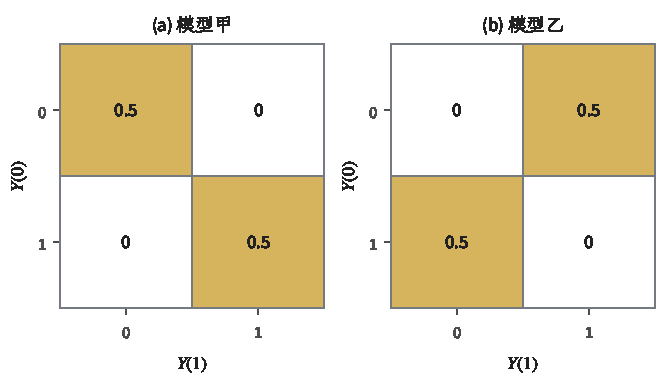
\includegraphics[width=\linewidth]{figures/01-mathematical-preliminaries/04-random-variables-distributions-and-causality/matplotlib/concepts-probability/causal-cross-world-couplings.pdf}
  \caption{相同干预边缘的两种跨世界配对。行对应\(Y(0)\)，列对应\(Y(1)\)，格内
  数字为联合概率；每张表的行和、列和均为\(1/2\)。甲的个体效应恒为零，乙的个体
  效应等概率取\(1,-1\)，两者ATE均为零。这是相容机制的教学构造，不是随机试验
  直接观察到的潜在结果联合表。}
  \label{fig:causal-cross-world-couplings}
\end{figure}

两套配对连完整随机试验的两组边缘也无法区分。要回答条件个体反事实，还需要关于
跨世界联合结构的机制限制，或具有适当稳定性、时间和携带效应假设的重复干预资料；
否则应保留相容范围。模型明确给定时可以用式
~\eqref{eq:causal-counterfactual-pushforward}计算，数据是否足以确定这套模型则是
第~\ref{sec:causal-effect-identification}节的另一个问题。

\subsection{目标约束下的行动补救}
\label{sec:causal-action-recourse}

反事实计算还可以反过来服务于行动选择：怎样以尽量低的代价，让同一个人的决策
达到目标？先区分两种看似相近的操作。对预测器\(\widehat y=f(x,t)\)，输入替换给出
\[
  f(x,1)-f(x,0).
\]
这只是已训练函数对字段变化的响应。若现实培训提高技能、同时占用工作时间，那么
只改“是否培训”一列而锁住技能和时间，通常不是任何可实施的行动结果。

\begin{definition}[因果行动补救]
  \label{def:causal-recourse}
  给定事实证据、可实施行动集合\(\mathcal A(x)\)、响应模型、行动成本\(c(a;x)\)
  与目标决策集合\(G\)，\term{行动补救}（algorithmic recourse）寻找能够使行动后
  的决策落入\(G\)的可行行动。因果行动补救用同一背景下的干预状态
  \(\bm V_a=F_M^a(\bm U)\)评价成功条件，并按机制重算所有受行动影响的状态。
\end{definition}

令\(d\)为最终决策规则。若事实唯一确定背景\(\bm u\)，优化形式为
\begin{equation}
  \min_{a\in\mathcal A(x)}c(a;x)
  \quad\text{使得}\quad d(F_M^a(\bm u))\in G.
  \label{eq:causal-recourse-objective}
\end{equation}
可行集合规定实际允许做什么，成本规定如何比较行动，成功约束规定要得到何种决策。
它们对应第~\ref{chap:optimization}章的约束优化接口，但不能只根据一个距离函数
代替全部三项。低输入距离不等于低行动成本；不可改变属性也不应成为行动建议。
若可行集合为空，应报告无法在当前约束下补救，而不是输出一个不可执行的最近点。

多数事实只能给出背景条件分布。给定可容许失败概率\(\alpha\in[0,1]\)，可以采用
概率型约束
\begin{equation}
  \mathbb P\bigl(d(F_M^a(\bm U))\in G\mid\bm E=\bm e\bigr)
  \geq1-\alpha.
  \label{eq:causal-recourse-probability}
\end{equation}
若背景空间带有指定拓扑，可选所用条件分布版本的支持
\[
  \mathcal S_{\bm e}
  =\operatorname{supp}P_{\bm U\mid\bm E=\bm e}.
\]
要求
\begin{equation}
  d(F_M^a(\bm u))\in G,\qquad \bm u\in\mathcal S_{\bm e},
  \label{eq:causal-recourse-robust}
\end{equation}
得到支持上的最坏情形保证。一般可测空间没有默认的拓扑支持，此时应明确给出候选
背景集合，而不是含糊使用“所有可能背景”。支持上逐点成功通常强于概率一成功，
因为它还涉及零概率点上的模型取值。

两点后验例子可以直接比较这些条件。若目标是\(Y_a\geq5\)，行动\(a\)的后验成功
概率为\(3/4\)，因此在\(\alpha=1/4\)时满足概率约束；但低类型背景的结果为\(2\)，
不能满足支持上的最坏情形保证。只挑高类型作为“代表背景”会漏掉这项风险。

补救也有时间和多人联动的边界。许多人同时接受建议可能改变价格、名额或审核规则；
决策系统更新后，原建议未必仍有效；资源竞争也可能使原先逐人可行的行动无法共同
执行。因此当前模型中存在一个成功行动，不等于建议已经通过现实可行性、持久性
或公平性验证。

\subsection{目标属性干预下的公平补救}
\label{sec:causal-fair-recourse}

达到有利决策与公平是两项要求。一个行动可能只在事实属性下成功，却在同一人的
替代属性世界里失败。要讨论这种差别，必须先说明哪些属性影响应当被排除，以及
替代属性在模型中如何改变其他状态。

令受保护属性为\(A\)，事实证据为\((X=x,A=a)\)。本小节的\(X\)泛指用于推断
背景的其他事实，可能包含属性的后继变量；它不再具有CATE中“处理前且保持不变”
的自动含义。事实中给定\(X=x\)，并不要求替代属性世界的\(X\)仍等于\(x\)。
\begin{definition}[反事实公平]
  \label{def:causal-counterfactual-fairness}
  在给定响应模型与预测规则下，\term{反事实公平}（counterfactual fairness）
  要求：对每个允许的替代属性\(a'\)和每个可测预测值集合\(B\)，以下等式对事实
  证据分布几乎处处的\((x,a)\)成立：
  \begin{equation}
    \begin{aligned}
      &\mathbb P(\widehat Y_{A\leftarrow a}\in B\mid X=x,A=a)\\
      &\qquad=
      \mathbb P(\widehat Y_{A\leftarrow a'}\in B\mid X=x,A=a).
    \end{aligned}
    \label{eq:causal-counterfactual-fairness}
  \end{equation}
  两个属性世界均使用同一个事实背景条件分布，并重新计算由属性影响的状态及预测。
\end{definition}

等式右侧仍以事实\(A=a\)为条件，而不是改用另一群人的证据\(A=a'\)。
只在输入表中替换\(A\)并固定其全部后继变量，检验的是另一个对象。属性干预在这里
是明确模型下的比较操作，也不表示应建议个人改变该属性。

把公平条件加入补救时，为避免与属性值混淆，记补救行动为\(b\)。
要求模型已经规定联合行动映射\(F_M^{b,A\leftarrow a'}\)：对每个属性世界，
保留同一个可比较的行动\(b\)，不对该世界偷偷重新选择更有利的行动。行动与属性
替换须互相兼容，且所比较世界中行动的可实施含义应明确。定义
\[
  \Pi_b^{a'}(B;x,a)
  =
  \mathbb P\bigl(
    d(F_M^{b,A\leftarrow a'}(\bm U))\in B
    \mid X=x,A=a
  \bigr).
\]
一种公平约束补救问题是
\begin{equation}
  \begin{aligned}
    \min_{b\in\mathcal A(x,a)}\quad &c(b;x,a)\\
    \text{使得}\quad
    &\Pi_b^a(G;x,a)\geq1-\alpha,\\
    &\Pi_b^{a'}(\cdot;x,a)=\Pi_b^a(\cdot;x,a)
      \quad\text{对每个允许的 }a'.
  \end{aligned}
  \label{eq:causal-fair-recourse-objective}
\end{equation}
第一项约束要求成功，第二项约束要求同背景的决策分布不随属性改变。也可以另选近似
公平或成本公平目标，但那会改变问题，不能把它们当作上述等式的自动结果。

\begin{example}[成功行动未必满足公平约束]
  \label{ex:causal-fair-recourse}
  设\(A\in\{0,1\}\)，自然培训量为\(B=0\)，资格分数与二元决策规则为
  \[
    K=U+A+B,\qquad d=\mathbb I\{K-2A\geq2\}.
  \]
  可行行动是把培训量设为\(b\in[0,3]\)，成本为\(c(b)=b\)，目标为\(d=1\)。
  已知事实\(A=0,B=0,K=1\)，于是\(U=1\)。在两个属性世界中施加同一行动，
  必须重算\(K\)，得到
  \[
    K_{b,A\leftarrow a'}=1+a'+b,\qquad
    d_{b,A\leftarrow a'}=\mathbb I\{1+b-a'\geq2\}.
  \]
  只要求事实属性下成功时，最小行动为\(b=1\)。但此时\(a'=0\)给决策\(1\)，
  \(a'=1\)给决策\(0\)，并不公平。若同时要求两个属性世界的二元决策相同且
  成功，则必须\(b\geq2\)，故最优行动为\(b=2\)。不行动时两个世界都失败，
  虽然决策相同，却不满足补救目标。
\end{example}

此例检验的是二元决策，不是内部实值分数\(K-2A\)；后者在两个属性世界中始终
相差\(1\)，任何培训量都不能让分数分布相同。公平对象、允许行动及预算都会影响
可行性。对一个已知个体成立的约束，也不自动保证面向所有人的推荐规则公平；
后者还需规定推荐怎样依赖事实，并对其目标人群几乎处处检验。

这些等式均以给定模型为条件。第~\ref{sec:causal-factual-counterfactual}节的
跨世界配对已经说明，相同干预边缘也可能给出不同条件反事实；由观测拟合出一套
生成规则，不等于公平或补救结论已被唯一识别。若多个模型与证据相容，应在该模型类
上报告结论范围。哪些属性或路径属于不应进入决策的因素，则是另需论证的规范选择。
\BookChapterRef{chap:trust-fairness}{第二卷“基础、理论和可信性”的“公平性”章}与
\BookChapterRef{chap:trust-interpretability}{第二卷“基础、理论和可信性”的“可解释性”章}
继续讨论公平要求、解释和补救的应用及现实验证边界。

\section{因果响应的推断}
\label{sec:causal-effect-identification}

前面把模型作为输入。现在模型未知，手中只有观察或试验资料，并有一组愿意接受的
机制假设。问题因而变为：这些资料与假设是否足以确定所选响应目标？
定义~\ref{def:statistics-identifiability}所述的识别思想在这里仍然适用，只是
模型索引从一般统计参数变成了完整生成机制。

记\(P_{\mathrm{obs}}^M\)为模型\(M\)在已声明观测制度下给出的可观测分布，
\(\tau(M)\)为目标。在允许模型类中，若
\[
  P_{\mathrm{obs}}^{M_1}=P_{\mathrm{obs}}^{M_2}
  \quad\Longrightarrow\quad \tau(M_1)=\tau(M_2),
\]
就称该目标\term{可识别}（identifiable）。可观测分布可以包括已完成的试验资料，
不必只包括自然观察。目标可识别也不要求模型每个组成部分都唯一确定。

这是总体层面的唯一性，须与有限样本估计、数值计算区分。估计用样本逼近总体量，
计算求出给定表达式或优化问题的答案。一个算法可以精确拟合全部观测条件分布，
却仍无法区分本章开头的两套机制；反过来，目标已有识别式，也不表示样本够多或
数值算法已经稳定。

\subsection{响应目标的点识别}
\label{sec:causal-point-identification}

要从事实数据恢复响应，关键是找到哪些可见单位可以代表目标行动下的结果。随机分配
直接建立可比性；观察研究则通常需要在足够的处理前信息下作比较。以下先把条件写成
潜在结果关系，不要求事先得到一张完全识别的因果图。

\subsubsection{随机分配下的边缘识别}
\label{sec:causal-randomized-identification}

若处理由独立随机装置分配，且两种处理都有正概率，则
\((Y(0),Y(1))\perp T\)。结合一致性，对任意可测集合\(B\)及
\(t\in\{0,1\}\)，有
\begin{equation}
  \mathbb P(Y(t)\in B)
  =
  \mathbb P(Y(t)\in B\mid T=t)
  =
  \mathbb P(Y\in B\mid T=t).
  \label{eq:causal-randomization-marginal-distribution}
\end{equation}
第一个等号来自随机分配，第二个来自实际处理与潜在结果的一致性；正概率保证右侧
有相应处理组。结果可积时，同一论证给出
\[
  \mathbb E[Y(t)]
  =\mathbb E[Y(t)\mid T=t]
  =\mathbb E[Y\mid T=t],
\]
所以两组均值差识别ATE。

式~\eqref{eq:causal-randomization-marginal-distribution}识别的是每个潜在结果的
完整边缘，不是\((Y(0),Y(1))\)的联合分布。第
~\ref{sec:causal-factual-counterfactual}节的两套配对因此仍与随机试验相容。
若实际分析存在失访、不依从、处理溢出或随机化后的样本筛选，应按真实目标重新检查
独立性和一致性。例如随机分配的邀请不等于实际参加培训，按参加者重新分组不会自动
继承原随机化。

\subsubsection{条件交换下的调整识别}
\label{sec:causal-adjustment-identification}

观察研究不能随意重排处理，但可以尝试用处理前\(X\)解释分配差异。这里的\(X\)
须在所比较处理下保持同一取值和含义，否则两组不再按共同背景分层。
\begin{definition}[条件交换性]
  \label{def:causal-conditional-exchangeability}
  对二元处理，\term{条件交换性}（conditional exchangeability）要求
  \begin{equation}
    (Y(0),Y(1))\perp T\mid X.
    \label{eq:causal-conditional-exchangeability}
  \end{equation}
\end{definition}
直观上，固定\(X\)后，进入处理组不再额外透露潜在结果的信息；例如\(X\)已经
包含需要控制的共同背景。这不同于概率论中样本序列在重排下分布不变的可交换性。
它涉及不能同时观察的结果，不能凭处理预测准确率或结果拟合误差验证。对单个边缘
目标，只需相应的\(Y(t)\perp T\mid X\)；上式是同时表达两种处理可比性的较强条件。

\begin{definition}[二元处理的支持重叠]
  \label{def:causal-overlap}
  记倾向概率为\(e(x)=\mathbb P(T=1\mid X=x)\)。对需要比较两种处理的目标总体，
  \term{支持重叠}（overlap），也称\term{正值性}（positivity），要求
  \begin{equation}
    0<e(x)<1,\qquad P_X\text{几乎处处}.
    \label{eq:causal-overlap}
  \end{equation}
\end{definition}
交换性解释参照人群为何可比，支持重叠保证参照确实存在。若某类人必然接受处理，
即使愿意假设其未处理潜在结果与分配条件独立，也没有该类人的未处理记录可用。

正值性随目标而定。识别\(\mathbb E[Y(1)]\)只需目标总体几乎处处有\(e(x)>0\)，
识别\(\mathbb E[Y(0)]\)只需\(e(x)<1\)，ATE才同时需要两侧条件。
对目标策略，只有它会使用的背景与行动组合需要被观测支持覆盖；目标总体以外的
背景和策略从不采取的行动不在要求内。若另换目标总体，其背景支持和跨总体条件
响应的可比性也要重新检查。

假设一致性、条件交换性、所需支持及潜在结果可积性成立。全期望先给出
\[
  \mathbb E[Y(t)]
  =\mathbb E_X[\mathbb E[Y(t)\mid X]].
\]
交换性允许在内层加入处理条件：
\[
  \mathbb E[Y(t)\mid X]
  =\mathbb E[Y(t)\mid T=t,X].
\]
正值性保证右侧在目标所需的背景上由相应处理组定义，一致性再将\(Y(t)\)换成
观察结果，得到调整公式
\begin{equation}
  \mathbb E[Y(t)]
  =\mathbb E_X[\mathbb E[Y\mid T=t,X]].
  \label{eq:causal-g-formula}
\end{equation}
令\(\mu_t(x)=\mathbb E[Y\mid T=t,X=x]\)，两式相减便有
\begin{equation}
  \tau=\mathbb E_X[\mu_1(X)-\mu_0(X)].
  \label{eq:causal-ate-adjustment}
\end{equation}
若把结果换成事件指示量，同样可以识别各干预边缘的事件概率。

同一目标还有逆概率表示。对处理组，由条件期望
\[
  \begin{aligned}
    \mathbb E\left[\frac{TY}{e(X)}\middle|X\right]
    &=
    \frac{\mathbb P(T=1\mid X)}{e(X)}
      \mathbb E[Y\mid T=1,X]\\
    &=\mu_1(X).
  \end{aligned}
\]
未处理组同理满足
\[
  \mathbb E\left[\frac{(1-T)Y}{1-e(X)}\middle|X\right]
  =\mu_0(X).
\]
可积性使这些期望存在，再取总体期望得到
\begin{equation}
  \tau=\mathbb E\left[
    \frac{TY}{e(X)}-\frac{(1-T)Y}{1-e(X)}
  \right].
  \label{eq:causal-ipw-identification}
\end{equation}
条件均值法先在层内比较再按总体平均；加权法给较少进入某处理的单位更大权重。
两者是同一识别关系的表示，不是两套彼此替代的因果假设。

下面把分配差异具体算出来。设\(X\in\{0,1\}\)表示处理前风险，
\(\mathbb P(X=1)=1/2\)，且
\[
  e(1)=0.8,\qquad e(0)=0.2.
\]
给定\(X\)后假设交换性成立，潜在结果均值取教学数值
\[
  \begin{array}{c|cc}
    &X=0&X=1\\ \hline
    \mathbb E[Y(0)\mid X]&0.1&0.5\\
    \mathbb E[Y(1)\mid X]&0.3&0.7
  \end{array}
\]
两层效应都为\(0.2\)，所以
\[
  \tau=\tfrac12(0.3-0.1)+\tfrac12(0.7-0.5)=0.2.
\]
自然处理中\(\mathbb P(T=1)=\tfrac12(0.8+0.2)=1/2\)，Bayes公式给出
\[
  \mathbb P(X=1\mid T=1)=0.8,\qquad
  \mathbb P(X=1\mid T=0)=0.2.
\]
于是观察到的两组均值为
\[
  \begin{aligned}
    \mathbb E[Y\mid T=1]&=0.8\times0.7+0.2\times0.3=0.62,\\
    \mathbb E[Y\mid T=0]&=0.2\times0.5+0.8\times0.1=0.18.
  \end{aligned}
\]
观测差为\(0.44\)，大于调整后的\(0.20\)，因为处理组中基础结果较高的高风险者
更多。按共同的\(P_X\)重新平均就恢复了所定义的总体效应。

这也说明三项假设各管什么。一致性连接观测和潜在结果，交换性允许同层比较，重叠
让每层都有所需的处理记录。遗漏未记录的病情可能破坏交换性；若\(e(1)=1\)，
高风险层的未处理结果完全缺失。相反，\(e(1)\)很接近但未等于\(1\)时，点识别
仍成立，只是有限样本中权重可能很大。选择哪些协变量足以支持调整，需要领域知识
或结构证书；第~\ref{sec:causal-backdoor-selection}节在建立图语义后给出一种
充分准则，这里并未假定该准则已经被验证。

\subsection{响应目标的部分识别}
\label{sec:causal-partial-identification-sensitivity}

若不愿接受完整交换性，或目标行动落入无数据的区域，仍可询问现有信息排除了哪些
答案。这就是\term{部分识别}（partial identification）：保留所有相容机制给出的
目标值，不用一个未经支持的点掩盖机制歧义。
\begin{definition}[识别集合]
  \label{def:causal-identified-set}
  设\(\mathcal M(P_{\mathrm{obs}})\)是与可观测分布及已声明假设相容的模型集合，
  目标为\(\tau(M)\)。其\term{识别集合}（identified set）是
  \begin{equation}
    \mathcal I(P_{\mathrm{obs}})
    =\{\tau(M):M\in\mathcal M(P_{\mathrm{obs}})\}.
    \label{eq:causal-identified-set}
  \end{equation}
\end{definition}
相容类为空意味着假设与观测不相容，并不是“目标取空值”。以下讨论相容类非空的
情形。一般识别集合可能由分离的点或区间组成；下确界和上确界只给区间包络，
不能保证包络内每个值可达。只有另外证明中间值可达，才能把整个区间称为识别集合。

\subsubsection{结果约束下的效应界}
\label{sec:causal-outcome-bounds}

先只保留一致性及结果范围\(0\leq Y(t)\leq1\)，不假设交换性。二元处理下，
\[
  \begin{aligned}
    \mathbb E[Y(1)]
    &=\mathbb E[TY(1)]+\mathbb E[(1-T)Y(1)]\\
    &=\mathbb E[TY]+\mathbb E[(1-T)Y(1)].
  \end{aligned}
\]
第一项已经观察到；第二项是未处理者接受处理后的结果。由范围约束，
\[
  0\leq\mathbb E[(1-T)Y(1)]\leq\mathbb P(T=0),
\]
所以
\begin{equation}
  \mathbb E[TY]\leq\mathbb E[Y(1)]
  \leq\mathbb E[TY]+\mathbb P(T=0).
  \label{eq:causal-bounded-outcome-y1}
\end{equation}
对另一处理，同样将
\(\mathbb E[Y(0)]=\mathbb E[(1-T)Y]+\mathbb E[TY(0)]\)分成可见与缺失部分，
得到
\begin{equation}
  \mathbb E[(1-T)Y]\leq\mathbb E[Y(0)]
  \leq\mathbb E[(1-T)Y]+\mathbb P(T=1).
  \label{eq:causal-bounded-outcome-y0}
\end{equation}
用第一式下端减第二式上端，反向组合得到上端：
\begin{equation}
  \begin{aligned}
    &\mathbb E[TY]-\mathbb E[(1-T)Y]-\mathbb P(T=1)
      \leq\tau\\
    &\qquad\leq
      \mathbb E[TY]+\mathbb P(T=0)-\mathbb E[(1-T)Y].
  \end{aligned}
  \label{eq:causal-manski-ate-bounds}
\end{equation}

界宽并不一定表示推导粗糙；它可能正是资料缺失造成的。
\begin{definition}[相容机制类中的锐界]
  \label{def:causal-sharp-bounds}
  对非空相容类\(\mathcal M(P_{\mathrm{obs}})\)与实值目标，若下界与上界分别等于
  \(\inf_{M\in\mathcal M}\tau(M)\)及\(\sup_{M\in\mathcal M}\tau(M)\)，就称为
  该机制类中的\term{锐界}（sharp bounds）。端点可以达到，也可以仅由相容
  机制序列任意逼近。
\end{definition}

式~\eqref{eq:causal-manski-ate-bounds}在当前不受其他限制的机制类中是锐的。
要达到下界，保持所有实际记录不变，令未处理者缺失的\(Y(1)=0\)，已处理者
缺失的\(Y(0)=1\)。要达到上界，则把这两类缺失结果分别设为\(1\)和\(0\)。
两种构造都满足一致性和结果范围，也不改变\(P_{\mathrm{obs}}\)。

中间值也可构造。独立抽取一个概率为\(\lambda\)的二元背景标记，按该标记选择
上端构造，否则选择下端构造；事实记录不变，只切换缺失结果的赋值。
混合机制的效应为\(\lambda\tau_{\mathrm{up}}+(1-\lambda)\tau_{\mathrm{low}}\)。
让\(\lambda\)遍历\([0,1]\)，便得到整个区间。这证明宽度不是代数松弛造成的。
若再要求个体单调性、平滑函数或特定跨世界结构，上述赋值可能不再允许，
锐界必须在新的模型类中重新计算。

\subsubsection{支持缺口下的效应与策略界}
\label{sec:causal-support-policy-bounds}

现在假设条件交换性可信，但双侧重叠只在协变量区域\(\mathcal O\)成立。用
\(\mathcal N\)表示目标总体中缺少某种处理的区域，两者不交且覆盖目标总体。
结果仍在\([0,1]\)时，条件效应\(\tau(x)\in[-1,1]\)，故
\[
  \tau=
  \mathbb E[\tau(X)\mathbb I\{X\in\mathcal O\}]
  +\mathbb E[\tau(X)\mathbb I\{X\in\mathcal N\}].
\]
第一项由调整式识别，第二项只能先按范围控制，得到
\begin{equation}
  \begin{aligned}
    &\mathbb E[\tau(X)\mathbb I\{X\in\mathcal O\}]
      -\mathbb P(X\in\mathcal N)\leq\tau\\
    &\qquad\leq
      \mathbb E[\tau(X)\mathbb I\{X\in\mathcal O\}]
      +\mathbb P(X\in\mathcal N).
  \end{aligned}
  \label{eq:causal-overlap-gap-bounds}
\end{equation}
这是一组有效界，未声称总是锐界；缺口区域中若仍观察到一种处理的结果，
利用这一侧均值还可能收紧。限制目标人群到\(\mathcal O\)可以点识别重叠人群效应，
但已经改变了目标总体。假设缺口内效应与邻近区域平滑、同号或落在更小范围，也能
收紧答案，却都是额外外推条件，不能由已覆盖部分的拟合优度证明。

单步策略评价需要的支持可以更少。沿用式~\eqref{eq:causal-policy-value}的有限
动作集合及目标策略\(\pi\)，记日志动作概率为
\(e_a(x)=\mathbb P(T=a\mid X=x)\)。假设对所有动作，
\(L\leq Y(a)\leq H\)，且一致性和给定\(X\)的交换性成立。若目标覆盖条件为
\[
  \pi(a\mid x)>0\quad\Longrightarrow\quad e_a(x)>0
\]
并在目标总体中几乎处处成立，则
\[
  \begin{aligned}
    \mathbb E\left[\frac{\pi(T\mid X)}{e_T(X)}Y\middle|X\right]
    &=
    \sum_{\substack{a\in\mathcal A\\e_a(X)>0}}
      e_a(X)\frac{\pi(a\mid X)}{e_a(X)}
      \mathbb E[Y\mid T=a,X]\\
    &=
    \sum_{a\in\mathcal A}\pi(a\mid X)\mathbb E[Y(a)\mid X].
  \end{aligned}
\]
对\(X\)取期望，得到
\begin{equation}
  V(\pi)=\mathbb E\left[\frac{\pi(T\mid X)}{e_T(X)}Y\right].
  \label{eq:causal-policy-value-weighting}
\end{equation}
这是第~\ref{sec:rv-change-measure}节换测度的一个因果用途：改变动作分配，
保留给定背景与动作的结果机制。权重只在日志实际可能选择的动作上求值，
覆盖条件使其余动作的目标概率为零，无须引入\(0/0\)约定。

覆盖失败时，记目标策略落入缺口的概率质量及已识别贡献为
\[
  \begin{aligned}
    r&=\mathbb E_X\left[\sum_{a:e_a(X)=0}\pi(a\mid X)\right],\\
    K&=\mathbb E_X\left[
      \sum_{a:e_a(X)>0}\pi(a\mid X)\mathbb E[Y\mid T=a,X]
    \right].
  \end{aligned}
\]
缺口部分的贡献在\([Lr,Hr]\)内，因而
\begin{equation}
  K+Lr\leq V(\pi)\leq K+Hr.
  \label{eq:causal-policy-value-bounds}
\end{equation}
两个策略的价值范围若完全分离，就能确定排序；若重叠，单独看边际范围未必能
判断。它们使用同一组未知潜在结果，不能把各自端点当作独立可选。
例如两策略完全相同时，无论各自的价值范围多宽，价值差都严格为零。
一般应对
\[
  V(\pi_1)-V(\pi_2)
  =
  \mathbb E_X\sum_a
    \bigl(\pi_1(a\mid X)-\pi_2(a\mid X)\bigr)\mathbb E[Y(a)\mid X]
\]
直接构造联合识别集合或上下界。拟合器对缺口给出的单一外推，不是额外的排序证据。

图~\ref{fig:causal-confounding-coverage}把混杂与覆盖分别数值化。左图回顾前面的
风险分层例子；右图另设结果范围为\([0,1]\)，已覆盖部分条件平均收益为\(0.6\)，
故\(K=0.6(1-r)\)。在\(r=0.2\)时，价值范围为\([0.48,0.68]\)。
宽度\(0.2\)来自缺口中的未知结果机制，不会因增加同一覆盖区域内的样本而消失。
\begin{figure*}[htbp]
  \centering
  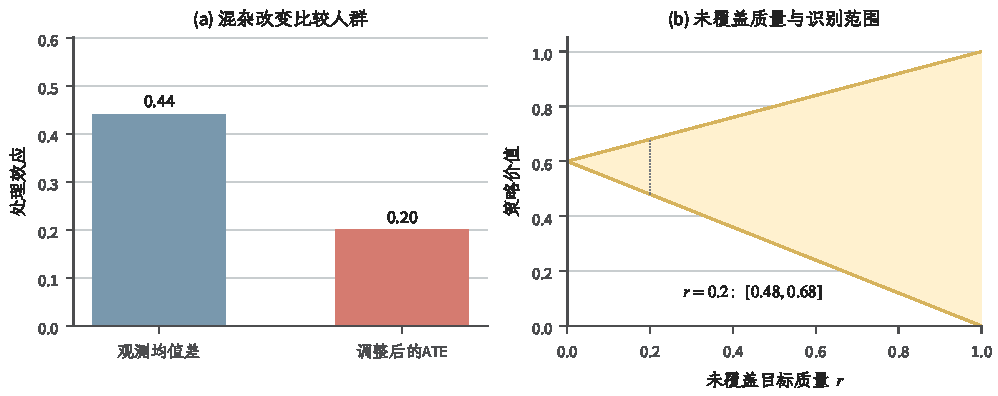
\includegraphics[width=\linewidth]{figures/01-mathematical-preliminaries/04-random-variables-distributions-and-causality/matplotlib/probability-discrete/causal-confounding-coverage.pdf}
  \caption{两个独立的教学构造。左图比较风险分层例子的观测均值差\(0.44\)与调整
  效应\(0.20\)。右图按式~\eqref{eq:causal-policy-value-bounds}绘制
  \([0.6(1-r),0.6(1-r)+r]\)。阴影为总体识别范围，不是抽样置信带；
  两个面板不表示同一数据集。}
  \label{fig:causal-confounding-coverage}
\end{figure*}

这里的策略只作一次行动。第~\ref{sec:decision-dynamic-programming}节建立序贯
策略后，必须逐时检查历史覆盖、时间变化的混杂及轨迹结果定义，不能把单步权重
直接套到整条轨迹。

\subsubsection{未观测混杂下的敏感性范围}
\label{sec:causal-sensitivity-ranges}

另一种缺口不是某类记录完全没有，而是相同已观测背景下仍存在未观测选择差异。
敏感性分析不强行断言该差异为零，而是规定其允许强度，检查结论随强度怎样变化。

先用一个最小线性模型定位偏差。设变量中心化，
\[
  T=\alpha U+\varepsilon_T,\qquad
  Y=\beta T+\gamma U+\varepsilon_Y,
\]
其中\(U,\varepsilon_T,\varepsilon_Y\)两两独立、方差有限，且
\(\operatorname{Var}(T)>0\)。理想设定\(T=t\)时，固定背景的结果对\(t\)的
导数为\(\beta\)。但只将\(Y\)对自然处理\(T\)作总体线性回归，得到
\begin{equation}
  \begin{aligned}
    \beta_{\mathrm{obs}}
    &=\frac{\operatorname{Cov}(T,Y)}{\operatorname{Var}(T)}\\
    &=\beta+
      \gamma\frac{\alpha\operatorname{Var}(U)}{\operatorname{Var}(T)}.
  \end{aligned}
  \label{eq:causal-linear-confounding-bias}
\end{equation}
这里用到了
\(\operatorname{Cov}(T,Y)=\beta\operatorname{Var}(T)
+\gamma\operatorname{Cov}(T,U)\)，以及
\(\operatorname{Cov}(T,U)=\alpha\operatorname{Var}(U)\)。
共同背景同时进入处理与结果，产生了第二项。若仅支持该偏差绝对值不超过
\(\Lambda\)，则
\(\beta\in[\beta_{\mathrm{obs}}-\Lambda,\beta_{\mathrm{obs}}+\Lambda]\)。
观测可以估计\(\beta_{\mathrm{obs}}\)，却不能在没有额外信息时把
\(\alpha,\gamma,\beta\)各自分开；改变函数形式也会改变敏感性参数的含义。

异质或非线性响应不一定有一个统一斜率修正量。仍记
\(\mu_t(x)=\mathbb E[Y\mid T=t,X=x]\)和\(e(x)=\mathbb P(T=1\mid X=x)\)。
在\(0<e(x)<1\)且相关条件期望有限时，定义选择偏差函数
\[
  \begin{aligned}
    b_1(x)&=\mathbb E[Y(1)\mid T=1,X=x]
            -\mathbb E[Y(1)\mid T=0,X=x],\\
    b_0(x)&=\mathbb E[Y(0)\mid T=1,X=x]
            -\mathbb E[Y(0)\mid T=0,X=x].
  \end{aligned}
\]
条件交换性蕴含\(b_1=b_0=0\)，但反过来只得到条件均值交换性，
不能推出完整潜在结果分布相同。比如两组都均值为零，一组恒等于零，另一组等概率
取\(1,-1\)，均值相同仍保留分布差异。

一致性给出
\(\mathbb E[Y(1)\mid T=1,X=x]=\mu_1(x)\)，再由全期望
\[
  \begin{aligned}
    \mathbb E[Y(1)\mid X=x]
    &=e(x)\mu_1(x)+(1-e(x))(\mu_1(x)-b_1(x))\\
    &=\mu_1(x)-(1-e(x))b_1(x).
  \end{aligned}
\]
另一侧有
\[
  \begin{aligned}
    \mathbb E[Y(0)\mid X=x]
    &=(1-e(x))\mu_0(x)+e(x)(\mu_0(x)+b_0(x))\\
    &=\mu_0(x)+e(x)b_0(x).
  \end{aligned}
\]
相减得到
\begin{equation}
  \tau(x)=\mu_1(x)-\mu_0(x)
  -(1-e(x))b_1(x)-e(x)b_0(x).
  \label{eq:causal-selection-bias-function}
\end{equation}
若领域知识仅支持
\(|b_1(x)|\leq\Gamma_1(x)\)及\(|b_0(x)|\leq\Gamma_0(x)\)，三角不等式给出
\begin{equation}
  \begin{aligned}
    \mu_1(x)-\mu_0(x)-\Delta(x)
    &\leq\tau(x)\\
    &\leq\mu_1(x)-\mu_0(x)+\Delta(x),
  \end{aligned}
  \label{eq:causal-sensitivity-bounds}
\end{equation}
其中\(\Delta(x)=(1-e(x))\Gamma_1(x)+e(x)\Gamma_0(x)\)。
重叠在目标总体几乎处处成立、潜在结果及相应控制量可积时，再对\(X\)平均便得到
ATE范围。该范围是当前偏差约束的有效包络；若还有限定结果范围或其他联合约束，
不能未经可达性检查就宣称它为锐界。

\(\Gamma_t\)是关于未观测差异的假设，不是样本自动生成的误差条。报告应展示在多大
强度下结论变号或越过决策阈值，而不只给一个恰好保留原结论的值。
其他有根据的假设也能缩小相容类。例如个体\term{单调性}（monotonicity）
\[
  Y(1)\geq Y(0)\quad\text{几乎必然}
\]
排除所有受损个体，故ATE至少为零，可以将有效下界提高到零。
它比“平均有益”更强。若已知个体效应位于\([-\rho,\rho]\)，支持缺口中的
\([-1,1]\)可换成更窄范围；平滑外推也必须作为新增机制限制声明。

跨环境资料可以提供另一种约束。若源环境有随机试验，目标环境给出协变量分布，
并假设条件效应在两环境相同，且目标协变量分布对源环境分布绝对连续，即源环境
的零概率背景集在目标环境中也为零概率，则
\[
  \tau_{\mathrm{target}}
  =\int\tau_{\mathrm{source}}(x)\,P_{X,\mathrm{target}}(\mathrm dx).
\]
这是条件效应稳定和目标覆盖共同给出的运输关系；在离散情形，覆盖要求目标中
出现的背景在源环境也有正概率。连续情形仅有拓扑支持包含还不够，应使用上述
绝对连续条件。它们都不是看到稳定预测关联就自动成立。
共同隐藏原因、选择过程或多个机制同步变化都可能产生稳定关联。

相容类也可用于第~\ref{sec:causal-counterfactual-recourse}节的反事实、补救与公平
目标。跨世界配对不同的模型可能同样解释试验边缘，却改变行动成功概率或公平判断。
此时应传播这些模型差异，而不是仅报告选定生成模型内的模拟精度。

\subsection{有限样本下的响应估计}
\label{sec:causal-response-estimation}

即使识别式成立，条件响应、处理概率与总体权重通常仍需从样本估计。比如调整法用
\(\widehat\mu_t\)代替\(\mu_t\)，再在目标背景样本上平均：
\[
  \widehat\tau
  =\frac1n\sum_{i=1}^n
    \bigl(\widehat\mu_1(X_i)-\widehat\mu_0(X_i)\bigr).
\]
这只是识别式的一种代入估计，不自动具有无偏性或某种收敛速度。拟合误差、目标样本
的抽样误差以及重复使用同一数据引入的依赖，仍须按第~\ref{sec:rv-inference}节
的估计与数据复用规则分析。采用样本拆分或交叉拟合时，应明确哪些样本拟合、哪些
样本评价，以及相应误差条件。

逆概率法还要估计倾向概率。很小但非零的真实概率允许总体识别，却可能使估计方差
很大；截断权重可改变偏差与方差，但不能被解释为凭空补足支持。更灵活的拟合器
或交叉拟合同样不能修复交换性错误。

部分识别时，估计对象可以是识别集合的端点或其外包络。识别集合在总体分布已知时
仍可能不是单点，表达机制歧义；\term{置信区间}来自有限样本，表达总体目标、
识别集合或端点的估计误差。对端点构造置信范围，还需按所用统计方法处理两个端点
共同的覆盖要求，不能把端点估计直接当作已知真界。

实际报告应分别列出相容机制留下的范围、抽样造成的不确定性，以及积分或优化中的
数值误差。增加样本主要改善第二项，改善算法主要影响第三项；改变设计、扩大目标
行动覆盖或加入可辩护的机制限制，才可能缩小第一项。尤其在效应符号或行动阈值附近，
应同时报告对支持处理、敏感性参数及目标总体选择的依赖。

\section{因果生成结构的表示}
\label{sec:causal-generating-structure}

前面把响应映射作为已知模型的接口，或把它放进与资料相容的候选类。现在打开这个
接口：培训先改变技能，技能再影响成绩，整体响应怎样由这些局部关系合成？需要记录
的不只有箭头，还包括每个变量的生成函数及未展开背景的联合分布。局部方程负责
产生数值，图负责记录输入关系；二者共同说明可以替换什么、替换后应重算什么。

\subsection{局部机制的结构方程表示}
\label{sec:causal-local-structural-equations}

把模型内需要解释的变量称为内生变量，把当前模型不再解释的背景称为外生变量。
“外生”是相对于模型边界而言，并不意味着这些量在现实中没有原因，也不自动意味着
它们彼此独立。进入某个变量生成函数的其他内生变量称为它的父变量，表示该局部机制
直接读取哪些输入。

\begin{definition}[无环结构因果模型]
  \label{def:causal-structural-model}
  本章的\term{结构因果模型}（structural causal model, SCM）由内生变量
  \(\bm V=(V_1,\ldots,V_d)\)的可测状态空间、外生背景
  \(\bm U=(U_1,\ldots,U_d)\)的联合分布及可测结构函数组成：
  \begin{equation}
    V_j=f_j(\operatorname{pa}_j,U_j),
    \qquad j=1,\ldots,d.
    \label{eq:causal-scm-definition}
  \end{equation}
  其中\(\operatorname{pa}_j\)收集进入第\(j\)个函数的其他内生变量。
  \term{无环}（acyclic）要求存在节点次序\(j_1,\ldots,j_d\)，使每个函数的
  内生输入都来自次序中更早的节点。外生分量可以相关。
\end{definition}

把每个内生变量画成节点，在\(V_k\)作为输入进入\(f_j\)时画箭头\(V_k\to V_j\)，
便得到有向无环图，简称DAG。上述求值次序已足以理解无环性，不需要先学习图排序
算法。SCM的箭头具有生成语义；若箭头只用于表示联合分布的条件分解，就不能据此
判断改变输入的后果\scite{math-pearl2009causality}

例如，培训\(T\)、技能\(M\)和成绩\(Y\)可以写成
\[
  T=f_T(U_T),\qquad
  M=\alpha T+U_M,\qquad
  Y=\beta T+\gamma M+U_Y.
\]
这里的直接输入关系为\(T\to M\)、\(T\to Y\)、\(M\to Y\)。若
\(U_T,U_M,U_Y\)相关，处理选择还可能与技能或成绩背景相联系；仅画出这三条内生边
不足以表示全部共同背景。要使用独立噪声DAG的概率规则，必须另行要求这些背景独立，
或把相关性的共同来源显式放进模型。

有限维模型可以把局部函数写成\(f_{j,\bm\theta_j}\)，并用
\(\bm\theta=(\bm\theta_1,\ldots,\bm\theta_d)\)汇集参数。上例的
\(\alpha,\beta,\gamma\)是局部作用参数；一般SCM则不必属于有限维函数族。
指定关系但不知道函数，或拟合函数却没有确定它的因果语义，都仍留下结构上的未知。

\subsection{局部机制的复合与响应生成}
\label{sec:causal-mechanism-composition}

有了局部方程，定义~\ref{def:causal-response-interface}假定的自然映射就可以
实际构造。无环次序让每一步只读取已经得到的值，因此既给出计算过程，也排除了
同一背景下出现多个自然解的歧义。

\begin{theorem}[无环机制的唯一可测响应]
  \label{thm:causal-acyclic-response}
  对定义~\ref{def:causal-structural-model}中的模型，每个背景
  \(\bm u\)唯一确定一组满足所有结构方程的内生取值。
  所得自然映射\(F_M:\mathcal U\to\mathcal V\)可测。将任意指定的一组方程
  替换为常量方程后，所得映射\(F_M^a\)同样存在、唯一且可测。
  对单变量理想干预，响应\((t,\bm u)\mapsto R_M(t,\bm u)\)联合可测。
\end{theorem}
\begin{proof}
  取符合无环性的次序\(j_1,\ldots,j_d\)。第一个变量没有内生父变量，
  因而\(v_{j_1}=f_{j_1}(u_{j_1})\)唯一确定，且是\(\bm u\)的可测函数。
  假设前\(k-1\)个变量已唯一确定为可测函数。第\(k\)个方程的父变量都在其中，
  将这些函数及\(u_{j_k}\)代入可测的\(f_{j_k}\)，便得到唯一且可测的
  \(v_{j_k}\)。归纳到\(d\)，得到满足全部方程的可测向量\(F_M(\bm u)\)。
  任何另一组解在第一个坐标都必须相同；逐坐标应用同一理由，便证明唯一性。

  常量替换只删除输入，不增加逆向依赖，原次序仍可使用。被替换坐标直接取行动
  指定值，其余坐标按同样归纳求出，从而得到\(F_M^a\)。
  若把处理值\(t\)也作为输入，被替换坐标是乘积空间上的投影
  \((t,\bm u)\mapsto t\)，其余步骤仍是可测函数的复合，因此
  \(F_M^{a(t)}(\bm u)\)及其结果坐标\(R_M(t,\bm u)\)联合可测。
\end{proof}

自然分布是\((F_M)_{\#}P_{\bm U}\)，干预分布是
\((F_M^a)_{\#}P_{\bm U}\)。两个推前共用同一个背景分布，只改变生成映射。
若理想干预值恰好等于该背景下的自然处理值，那么自然解也满足替换后的全部方程；
由唯一性，两组解相同。这也证明了这种构造中的一致性，而不只是另行假定
\(Y=Y(T)\)。

若结果方程为\(Y=f_Y(T,X,U_Y)\)，且\(X\)不受处理干预影响，则
\begin{equation}
  Y(t)=f_Y(t,X,U_Y).
  \label{eq:causal-scm-potential-outcome}
\end{equation}
因此\(\mathcal L(Y(t))=\mathcal L(Y\mid\operatorname{do}(T=t))\)。
若结果还依赖处理会改变的技能\(M\)，则必须先重算\(M(t)\)，不能仍代入事实技能。
对上面的线性机制，
\[
  M(t)=\alpha t+U_M,\qquad
  Y(t)=(\beta+\gamma\alpha)t+\gamma U_M+U_Y,
\]
所以整体响应导数为\(\beta+\gamma\alpha\)，不只是局部结果方程中固定\(M\)
时的偏导数\(\beta\)。取\(\alpha=2,\beta=1,\gamma=3\)，增加一单位培训使成绩
增加\(7\)，其中直接贡献为\(1\)，经技能传递的贡献为\(6\)。
对可微的非线性机制\(M=f_M(T,U_M)\)、\(Y=f_Y(T,M,U_Y)\)，链式法则给出
\[
  \frac{\partial R_M(t,\bm u)}{\partial t}
  =
  \frac{\partial f_Y}{\partial t}
  +
  \frac{\partial f_Y}{\partial m}
  \frac{\partial f_M}{\partial t},
\]
各偏导数均在该背景的干预取值处计算。这连接了第~\ref{sec:causal-local-response}节
的整体局部变化与本节的局部方程；对它再作总体平均，仍须检查导数与积分交换条件。

在外生噪声相互独立时，还可以用局部概率核表达同一计算。记
\[
  K_j(B\mid\bm v_{\operatorname{pa}_j})
  =
  \mathbb P\bigl(f_j(\bm v_{\operatorname{pa}_j},U_j)\in B\bigr).
\]
每个核都由机制及噪声分布指定，沿无环次序复合这些核便得到联合分布。独立性保证
当前噪声不会被已经生成的变量额外筛选。若这些核具有质量函数或密度，则
\[
  p(\bm v)=\prod_{j=1}^d p(v_j\mid\operatorname{pa}_j).
\]
理想干预把处理核换成点质量，其余核保持原样，于是得到\term{截断分解}
\begin{equation}
  p(\bm v_{-T}\mid\operatorname{do}(T=t))
  =
  \prod_{j:V_j\ne T}
  p(v_j\mid\operatorname{pa}_j)\big|_{T=t}.
  \label{eq:causal-truncated-factorization}
\end{equation}
这里\(\bm v_{-T}\)表示删除处理坐标后的变量集合。公式来自机制替换，不是对
任意概率分解删除一个因子都能得到因果分布。外生噪声相关时，上述独立核复合一般
不成立；应回到完整背景的推前，或显式展开相关来源。

局部因子必须使用结构机制指定的版本。观测分布只在父变量实际出现的支持上确定
条件分布；干预若产生了未见过的父变量组合，机制可以给出答案，但资料未必能识别
该答案。随意补一个支持外的条件密度，不会把模型外推变成数据结论。

对简单结构\(X\to T\)、\(X\to Y\)、\(T\to Y\)，用独立的新随机量按
\(q(t\mid x)\)分配处理，并保持其余独立噪声机制不变，得到
\begin{equation}
  p^q(x,t,y)=p(x)q(t\mid x)p(y\mid t,x).
  \label{eq:causal-stochastic-intervention}
\end{equation}
这正是第~\ref{sec:causal-intervention-potential-outcomes}节随机干预构造的局部
表达。确定性策略用点质量核表示，不必假装它有通常的Lebesgue密度。
策略若同时改变参与人群、结果测量或其他机制，就不能只替换处理因子。
更一般的机制替换也需要保证修改后的方程有明确解；添加依赖关系时，原无环次序
可能不再适用。

循环方程说明这一边界并非形式问题。例如\(V_1=V_2+1,V_2=V_1\)无解，而
\(V_1=V_2,V_2=V_1\)有无穷多组解。反馈系统可能需要动态演化、平衡选择或额外
唯一性条件，不能直接套用本节递归证明。

\subsection{变量关系的图表示与调整条件}
\label{sec:causal-graph-adjustment}

完整求解SCM可以得到响应，但有时只需回答一个较窄的问题：哪些变量适合用来调整
处理组之间的背景差异？图保留直接输入关系而暂时略去具体函数，因而能在一类机制
上共同作出判断。下面先看三种局部关系，再检查全图路径，最后把判断接到已经证明
的调整公式。

\subsubsection{局部因果关系与调整影响}
\label{sec:causal-local-path-patterns}

结构\(T\leftarrow X\to Y\)把\(X\)称为\(T\)与\(Y\)的
\term{共同原因}（common cause）。即使处理并不影响结果，不同\(X\)人群接受
处理的比例不同，也会使\(T,Y\)在自然记录中相关。这是混杂产生的一种方式。
第~\ref{sec:causal-adjustment-identification}节的风险分层算例正是通过在同一背景层
比较，再用同一目标权重平均，消除了由两组构成不同造成的差异。

结构\(T\to M\to Y\)中的\(M\)是\term{中介变量}（mediator）：处理对结果的
一部分影响经过它传递。若目标是总效应，固定\(M\)会阻断这部分变化；若研究同时
设定\(T=t,M=m\)的响应，则需明确这是不同的联合干预。
在线性例子中，固定中介后的处理系数为\(\beta\)，让中介随处理变化的总系数为
\(\beta+\gamma\alpha\)。这并不建立一般路径效应的识别公式，只说明两种目标不同。

结构\(T\to C\leftarrow Y\)中的\(C\)是\term{碰撞点}（collider），两条箭头
在此相遇。不以\(C\)筛选时，这条路径本身不要求两端相关；一旦给定\(C\)，却可能
引入关联。例如两个独立能力共同决定总分，入选要求总分超过阈值且两项能力可以
补偿，那么入选者中一项能力较弱的人往往需要另一项更强。若入选规则改成两项能力
分别超过各自阈值，这种负关联未必出现。关系的方向取决于选择机制，不能把选择
后的相关解释为一种能力造成另一种能力。

图~\ref{fig:causal-local-path-patterns}中的双边框表示中间变量被加入条件集。
共同原因和中介在该路径上都是非碰撞点，给定后会关闭路径；碰撞点的行为相反。
这解释了为何“控制更多变量”不是普遍有效的做法，也预告了局部路径能否关闭与
全图是否仍有其他路径是两件事。
\begin{figure*}[htbp]
  \centering
  \begin{tikzpicture}[figure picture,x=1mm,y=1mm,
  causalnode/.style={circle,draw=FigureStroke,fill=none,line width=1pt,
    minimum size=7mm,inner sep=0pt,font=\figurefont\mdseries\footnotesize},
  conditionednode/.style={causalnode,draw=FigureYellow,
    double=white,double distance=0.7pt},
  causaledge/.style={-{Stealth[length=2.2mm,width=1.4mm]},
    draw=FigureStroke,line width=1.1pt},
  paneltitle/.style={font=\figurefont\mdseries\footnotesize,text=FigureInk},
  panellabel/.style={font=\figurefont\mdseries\small,text=FigureInk},
  note/.style={font=\figurefont\mdseries\footnotesize,
    text=FigureMuted,align=center,fill=none}]
  \path[use as bounding box] (0,-10) rectangle (169,38);
  \draw[FigureGrid,line width=0.6pt] (56,-8)--(56,36);
  \draw[FigureGrid,line width=0.6pt] (112,-8)--(112,36);

  \node[panellabel,anchor=west] at (1,33) {(a)};
  \node[paneltitle] at (28,33) {共同原因};
  \node[conditionednode] (fork-x) at (28,22) {\(X\)};
  \node[causalnode] (fork-t) at (13,11) {\(T\)};
  \node[causalnode] (fork-y) at (43,11) {\(Y\)};
  \draw[causaledge] (fork-x)--(fork-t);
  \draw[causaledge] (fork-x)--(fork-y);
  \node[note] at (28,-3) {给定\(X\)时关闭路径};

  \node[panellabel,anchor=west] at (57,33) {(b)};
  \node[paneltitle] at (84,33) {中介链};
  \node[causalnode] (chain-t) at (67,16) {\(T\)};
  \node[conditionednode] (chain-m) at (84,16) {\(M\)};
  \node[causalnode] (chain-y) at (101,16) {\(Y\)};
  \draw[causaledge] (chain-t)--(chain-m);
  \draw[causaledge] (chain-m)--(chain-y);
  \node[note] at (84,-3) {给定\(M\)时关闭路径};

  \node[panellabel,anchor=west] at (113,33) {(c)};
  \node[paneltitle] at (140,33) {碰撞点};
  \node[causalnode] (collider-t) at (125,22) {\(T\)};
  \node[causalnode] (collider-y) at (155,22) {\(Y\)};
  \node[conditionednode] (collider-c) at (140,11) {\(C\)};
  \draw[causaledge] (collider-t)--(collider-c);
  \draw[causaledge] (collider-y)--(collider-c);
  \node[note] at (140,-3) {不给定时关闭\\给定\(C\)时打开};
\end{tikzpicture}

  \caption{共同原因、中介与碰撞点的局部路径。双边框表示节点已加入条件集。
  共同原因和中介是非碰撞点，给定后关闭这条路径；给定碰撞点则打开原本关闭的
  路径。路径打开表示图不再保证相应独立性，并不指定相关的大小或正负。}
  \label{fig:causal-local-path-patterns}
\end{figure*}

\subsubsection{全图路径分离与概率约束}
\label{sec:causal-global-path-separation}

较大图中，关闭一个局部片段仍可能留下另一条联系。设
\(\mathcal G=(V,E)\)是有向无环图，\(V\)是节点集、\(E\)是有向边集。
下面沿用定义~\ref{def:graph-theory-d-separation}的图分离判据，
在生成模型中解释它怎样约束随机变量的条件独立。路径仍指底层图中相邻且互不重复
的节点序列，有向路径才要求沿箭头前进；祖先和后代均不包括节点自身。

\begin{definition}[图分离与概率独立的记号]
  \label{def:causal-d-separation}
  对两两不交的节点集\(A,B,S\)，其中\(A,B\)非空，
  \(A\perp_{\mathcal G}B\mid S\)表示图中连接\(A,B\)的每条路径都被\(S\)
  阻断；活跃路径的碰撞与非碰撞规则沿用定义~\ref{def:graph-theory-d-separation}。
  若各节点承载随机变量，\(X_A\perp X_B\mid X_S\)则表示给定\(X_S\)后，
  \(X_A,X_B\)的条件联合分布分解为条件边缘分布的乘积。
  前一个记号只依赖图，后一个记号依赖概率分布；二者之间的联系需要模型假设。
\end{definition}

碰撞点是相对于某一条路径而言的，同一节点在不同路径上可以扮演不同角色。
给定其后代也可能传回选择信息，因此不能只检查碰撞点本身是否在条件集。
以同时含有
\[
  X\to M\to Y,\qquad X\to C\leftarrow Y,\qquad C\to D
\]
的图为例，\(X,Y\)之间有经过\(M\)和经过\(C\)的两条路径。四种条件集给出
不同判断：
\begin{itemize}
  \item \(S=\varnothing\)：经过\(M\)的链活跃，经过\(C\)的碰撞路径关闭，
  因而两端仍然d-连接。
  \item \(S=\{M\}\)：链被关闭，碰撞路径也仍关闭，所以
  \(X\perp_{\mathcal G}Y\mid M\)。
  \item \(S=\{M,C\}\)：链仍关闭，但给定碰撞点打开下方路径，两端重新d-连接。
  \item \(S=\{M,D\}\)：给定碰撞点的后代也打开下方路径，两端同样d-连接。
\end{itemize}
图~\ref{fig:causal-d-separation-paths}显示第二种情形。这个例子在本章即可逐路
检查；一般路径、分离与图分解的计算工具已在第~\ref{chap:graph-theory}章建立。
\begin{figure}[htbp]
  \centering
  \begin{tikzpicture}[figure picture,x=1mm,y=1mm,
  causalnode/.style={circle,draw=FigureStroke,fill=none,line width=1pt,
    minimum size=7mm,inner sep=0pt,font=\figurefont\mdseries\footnotesize},
  conditionednode/.style={causalnode,draw=FigureYellow,
    double=white,double distance=0.7pt},
  causaledge/.style={-{Stealth[length=2.2mm,width=1.4mm]},
    draw=FigureStroke,line width=1.1pt},
  note/.style={font=\figurefont\mdseries\footnotesize,
    text=FigureMuted,align=center,fill=none}]
  \path[use as bounding box] (0,-22) rectangle (112,32);
  \node[note,text=FigureInk] at (56,27) {条件集\(S=\{M\}\)};
  \node[causalnode] (dsep-x) at (16,14) {\(X\)};
  \node[conditionednode] (dsep-m) at (56,14) {\(M\)};
  \node[causalnode] (dsep-y) at (96,14) {\(Y\)};
  \node[causalnode] (dsep-c) at (56,-1) {\(C\)};
  \node[causalnode] (dsep-d) at (56,-16) {\(D\)};
  \draw[causaledge] (dsep-x)--(dsep-m);
  \draw[causaledge] (dsep-m)--(dsep-y);
  \draw[causaledge] (dsep-x)--(dsep-c);
  \draw[causaledge] (dsep-y)--(dsep-c);
  \draw[causaledge] (dsep-c)--(dsep-d);
\end{tikzpicture}

  \caption{多条路径下的d-分离。双边框节点\(M\)属于条件集，上方链式路径关闭；
  碰撞点\(C\)及其后代\(D\)都未给定，下方路径也关闭。若再把\(C\)或\(D\)
  加入条件集，下方路径就会打开，说明增加条件可能破坏原有的分离。}
  \label{fig:causal-d-separation-paths}
\end{figure}
\FloatBarrier

\begin{definition}[因果Markov性]
  \label{def:causal-markov-property}
  分布\(P\)相对于因果DAG \(\mathcal G\)满足\term{因果Markov性}
  （causal Markov property），是指对任意两两不交的节点集\(A,B,S\)，
  \[
    A\perp_{\mathcal G}B\mid S
    \quad\Longrightarrow\quad
    \bm V_A\perp\bm V_B\mid\bm V_S.
  \]
  其中\(\bm V_A,\bm V_B,\bm V_S\)分别收集对应节点的随机变量。
\end{definition}

左边是图规则，右边是分布性质。因果Markov性把前者的阻断结论转成条件独立；
它没有说d-连接一定产生统计依赖，也没有从观测独立直接反推箭头。它与时序过程
“给定当前状态后无须更早历史”的Markov性质使用不同对象和条件集，不能只因名称
相同就互相代入。

对DAG，这一全局表述等价于局部表述：每个变量在给定父变量后，与其非后代中除
自身和父变量外的变量条件独立。独立外生噪声的无环SCM满足这一性质。
直观上，非后代及父变量不读取当前节点的独立噪声；给定父变量后，当前变量剩下
的随机性就来自这一噪声。对局部核乘积，按逆向求值次序逐个积分掉无关后代，
每次被消去的条件核积分为一，由此保留所需的局部条件因子。分解与d-分离的
全局对应是DAG的标准结论\scite{math-pearl2009causality}
图分解与消元工具见第~\ref{chap:graph-theory}章；把图分离转成概率独立，
还需要这里的DAG分解或生成机制条件，不能只凭连接结构推出。
若背景相关而共同来源没有入图，不能仍对这个省略后的DAG直接宣称因果Markov性。

\subsubsection{后门条件下的调整变量选择}
\label{sec:causal-backdoor-selection}

第~\ref{sec:causal-adjustment-identification}节直接假定条件交换性，再证明调整
识别。现在可以反过来问：一张已经具有生成语义的图，能否为调整变量的选择提供
充分依据？从\(T\)到\(Y\)且第一条边指向\(T\)的路径称为
\term{后门路径}（back-door path），它从处理的自然生成来源进入比较，而非沿
处理对结果的有向作用出发。

\begin{definition}[单处理、单结果的后门准则]
  \label{def:causal-backdoor-criterion}
  设\(T,Y\)是因果DAG中的不同节点，\(Z\)与\(\{T,Y\}\)不交。若\(Z\)
  不含\(T\)的后代，且给定\(Z\)阻断所有从\(T\)到\(Y\)、第一条边指向
  \(T\)的路径，则称\(Z\)满足相对于\((T,Y)\)的
  \term{后门准则}（back-door criterion）。
\end{definition}

阻断按定义~\ref{def:causal-d-separation}判断，把碰撞点放进\(Z\)可能打开
原本关闭的路径。最基本的代表图为\(Z\to T,Z\to Y,T\to Y\)，独立噪声机制给出
\[
  p(z,t,y)=p(z)p(t\mid z)p(y\mid t,z).
\]
将处理机制替换为常量\(t\)后，
\(p(z,y\mid\operatorname{do}(T=t))=p(z)p(y\mid t,z)\)。再对背景积分，得到
\begin{equation}
  p(y\mid\operatorname{do}(T=t))
  =
  \int p(y\mid t,z)p(z)\,\mathrm dz.
  \label{eq:causal-backdoor-adjustment}
\end{equation}
离散背景用求和，一般空间用对\(P_Z\)的核积分。对结果再取期望，就回到
式~\eqref{eq:causal-g-formula}的调整表示。

一般后门准则在独立噪声无环SCM、图正确包含相关共同原因且干预保留其他机制的
条件下，给出同样的调整结论\scite{math-pearl2009causality}
阻断全部后门路径排除了自然处理选择沿这些路径携带的背景差异，非后代条件保证
用于平均的\(Z\)不先被行动改变。这些是生成结构对交换性的充分支持，而不是只由
一个观测分布满足Markov性就能推出的干预结论。即使图条件成立，要从观测资料
确定积分中的局部响应，还需要目标总体内所用处理的支持条件；图不会填补空白
协变量--处理组合。

三个局部图可以核对变量角色。在\(T\leftarrow X\to Y\)中，\(X\)关闭后门；
在\(T\to M\to Y\)中，\(M\)是后代，固定它会改变总效应目标；
在\(T\to C\leftarrow Y\)中，空条件集已经关闭碰撞路径，加入\(C\)反而打开它。
因此，处理前测量、与结果相关或能提高预测精度，都不是充分的调整标准。
后门准则是充分条件，不是识别的必要条件；它不适用时，随机设计、其他识别规则
或更具体的机制假设仍可能确定所选目标。

\section{因果生成结构的推断}
\label{sec:causal-structure-discovery}

此前给定图和局部机制，便能生成响应或支持调整。实际研究还可能不知道哪些变量
直接相连，也不知道相连以后怎样传递变化。前一项是变量关系的推断，后一项是局部
机制的推断；它们共同决定响应，但所需信息并不相同。一个模型能拟合观测数据，
不代表它的箭头、结构函数和同背景反事实都已经被唯一确定。

\subsection{变量关系的推断}
\label{sec:causal-relation-inference}

从图推出分布约束与从分布反推图，是方向相反的两项任务。要用条件独立排除候选
关系，需要说明哪些独立是真正的结构阻断，哪些可能来自参数抵消。资料制度也很
重要：同分布观察、受控干预和不同环境提供的限制不一样。

\subsubsection{观测资料下的关系识别}
\label{sec:causal-observational-structure}

\begin{definition}[相对于DAG的忠实性]
  \label{def:causal-faithfulness}
  分布\(P\)相对于DAG \(\mathcal G\)满足\term{忠实性}（faithfulness），若对
  任意两两不交的节点集\(A,B,S\)，
  \[
    \bm V_A\perp\bm V_B\mid\bm V_S
    \quad\Longrightarrow\quad
    A\perp_{\mathcal G}B\mid S.
  \]
\end{definition}
忠实性要求分布中出现的条件独立能由图结构解释，不是由特殊参数抵消、确定性
约束或未处理的误差相关造成。因果Markov性给出正向蕴含，忠实性补上反向蕴含，
两者不能互相替代。

例如，设\(X,U_M,U_Y\)相互独立，
\(M=\alpha X+U_M\)，\(Y=\beta X+\gamma M+U_Y\)。
当\(\alpha,\gamma\ne0\)且\(\beta=-\gamma\alpha\)时，
\(Y=\gamma U_M+U_Y\)与\(X\)独立，但图中直接路径\(X\to Y\)及
\(X\to M\to Y\)都存在。两条贡献恰好抵消，说明无环与独立噪声并不自动保证
忠实性。接近这种抵消时，非零依赖还可能非常弱，有限样本中难以检出。

只考察三个节点且没有其他路径时，链
\(X\to Z\to Y\)、反向链\(X\leftarrow Z\leftarrow Y\)和共同原因
\(X\leftarrow Z\to Y\)都蕴含
\[
  X\perp Y\mid Z,
\]
却一般不蕴含\(X\perp Y\)。条件独立模式无法区分中间变量在传递作用还是造成
共同变化。碰撞结构\(X\to Z\leftarrow Y\)则蕴含\(X\perp Y\)，给定中间
节点后可能相关；加上忠实性，才能把这种模式差别用作反向辨识的依据。
这回用了图~\ref{fig:causal-local-path-patterns}，但大图还必须检查所有其他路径。

\begin{definition}[Markov等价与等价类]
  \label{def:causal-markov-equivalence}
  同一节点集上的两张DAG若具有完全相同的d-分离关系，就称它们
  \term{Markov等价}（Markov equivalent）。
  与给定图Markov等价的全部DAG组成其
  \term{Markov等价类}（Markov equivalence class, MEC）。
\end{definition}

图的\term{骨架}（skeleton）是忽略箭头方向后的邻接关系。
\term{无屏蔽碰撞结构}（unshielded collider）指
\(X\to Z\leftarrow Y\)，并且两端\(X,Y\)不相邻。没有两端的直接边，才使
这个局部碰撞的差异能够通过两端的分离关系表现出来。
标准判据是：两张DAG Markov等价，当且仅当具有相同骨架和相同无屏蔽碰撞结构
\scite{pgm-structure-learning-chickering2002}

判据的必要性可以直接从全部路径证明。先说明DAG中任意两个非相邻节点都有一个
不含端点的d-分离集。选其中一个节点\(v\)，使另一个节点\(w\)不是它的后代；
无环性保证至少有这样一个选择。令条件集为\(v\)的父节点集。
任意从\(v\)到\(w\)的路径若第一条边指向\(v\)，就经过一个父节点；因两端
不相邻，该父节点是内部非碰撞点，路径被阻断。
若第一条边从\(v\)向外，路径不可能一直沿箭头到达非后代\(w\)。沿路径第一次
改变箭头方向时，出现一个碰撞点\(c\)，此前的有向前缀说明\(c\)是\(v\)的
后代。\(c\)及其任何后代都不可能成为\(v\)的父节点，否则形成有向环；
故这个碰撞点没有被条件集打开，路径仍被阻断。两类覆盖了全部路径。
相邻节点之间的单边路径则没有内部点，不可能被任何不含端点的条件集阻断。
因此，骨架不同必导致d-分离关系不同。

再考虑同一骨架上的无屏蔽三点结构\(X-Z-Y\)。两端不相邻，按上段存在分离集。
若\(Z\)不是碰撞点，任何分离集都必须包含\(Z\)，否则长度为二的这条路径
仍然活跃；若\(Z\)是碰撞点，任何分离集都不能包含\(Z\)，否则该路径被打开。
因此，中点碰撞状态不同也必然改变d-分离关系。其他路径可能增加分离要求，却
不会消除这条长度为二的路径对每个分离集施加的限制。

充分性需要控制所有较长路径，这里引用完整结构判据，不把上述必要性论证冒充
双向证明\scite{pgm-structure-learning-chickering2002}
理解等价类内部的方向变化还可借助\term{覆盖边}（covered edge）：边
\(X\to Y\)若满足
\[
  \operatorname{pa}(Y)=\operatorname{pa}(X)\cup\{X\},
\]
便是覆盖边，这里\(\operatorname{pa}(X)\)表示父节点集合。
覆盖边反转定理说明，反转这种边后仍为DAG，并保持全部d-分离关系
\scite{pgm-structure-learning-chickering2002}
从局部因子看，对给定共同父变量，这一步把
\[
  p(x\mid\operatorname{pa}(X))
  p(y\mid x,\operatorname{pa}(X))
  =
  p(y\mid\operatorname{pa}(X))
  p(x\mid y,\operatorname{pa}(X))
\]
重新分解，不改变两变量的条件联合分布。因子应取相容的条件版本；这个等式解释
分布重参数化，却没有单独证明全图等价，更没有证明两张指定图之间存在变换序列。
完整变换定理进一步保证，任意两张已知Markov等价的DAG，可以经有限次覆盖边
反转相互到达，每个中间图都保持无环且等价。这是等价类内的可达性结论，不能
代替结构判据的充分性证明\scite{pgm-structure-learning-chickering2002}

等价类可以用部分有向图表示：全部等价图都同意的方向保留箭头，其余边保持无向。
在因果Markov性、忠实性、无环和无潜在混杂等条件下，纯观测条件独立信息一般
只能识别这样的等价类。输出一条无向边并非一定表示算法未完成；它可能记录总体
观测分布本身无法决定的方向。增加同分布样本能改善独立性判断，却不会制造类内
所缺少的方向信息。

这里还隐含了变量覆盖。所有相关共同原因都已纳入可观测变量时，称满足因果充分性。
潜在共同原因能让两个可观测节点相关，却不应被硬解释成其中一个直接导致另一个。
允许潜在混杂或选择后，输出往往需要扩大到带不同端点标记的部分图，分别表示
已确定的祖先关系、可能方向和无法排除的隐藏共同原因。测量误差以及按碰撞点
选择样本也会改变独立模式，不应一律视为新增因果边。

有限样本中的关系发现还要通过检验或评分近似总体判断。以
\(H_0:V_i\perp V_j\mid\bm V_S\)为原假设，若约束型算法在未拒绝独立时
删除候选边，那么第一类错误把真实独立误判为依赖，可能保留虚假边；
第二类错误把实际依赖误判为独立，可能删除真实边。后续搜索与定向会传播错误，
评分型算法则不能直接套用这组对应。高维条件集减少每层有效样本，近忠实边界上
的弱依赖尤其难判断。结构学习的一致性必须同时说明总体的Markov与忠实条件、
检验或评分的渐近性质、候选图范围，以及搜索能否达到目标；一张确定输出图
不代表因果方向已经唯一。

\subsubsection{干预与环境变化下的方向识别}
\label{sec:causal-interventional-structure}

要打破观测方向歧义，需要增加具有不同约束的信息。理想干预切断目标变量的原
进入机制：若随机设置\(X\)后，\(Y\)的分布随设置值改变，在其余机制不变、
行动确实只作用于\(X\)的模型中，这支持\(X\)位于\(Y\)的上游。反之，没有
观察到分布改变并不自动排除作用，机制抵消、剂量范围或检验能力都可能影响判断。
对多个节点施加适当干预可缩小观测等价类，但能缩小到什么程度取决于干预覆盖。

这一证据必须按实际执行解释。干预目标未知、执行不完全，或干预同时改变测量、
选择和其他机制时，都应将这些不确定性纳入模型。不能把“鼓励参加培训”无条件
等同于“把培训处理设为指定值”，也不能把伴随整套制度改变的干预解释成单个
节点的理想替换。

不同环境也可能提供方向限制。设环境标签为\(E\)，若假定环境只改变输入\(X\)
的分布，而机制\(Y=f_Y(X,U_Y)\)及独立噪声\(U_Y\)的分布保持不变，那么
各环境在共同支持上的\(P(Y\mid X,E=e)\)应相同；反向条件分布
\(P(X\mid Y,E=e)\)却可能随输入分布变化。这里稳定性来自已声明的生成假设，
并非看到一个稳定条件分布就证明了箭头。

潜在共同原因可以在所有已观察环境中稳定，环境变化也可能太弱，未能打破错误
方向；选择规则同步变化还可能制造稳定关联。应分别说明哪些背景分布或局部
机制允许改变，哪些保持不变，环境是否直接影响结果，以及稳定性究竟是模型
假设、检验对象还是经验线索。机制知识和对隐藏混杂、弱依赖、选择过程的
敏感性分析，共同限制候选关系，不能由增加同分布样本替代。

对于反馈环、随时间改变的机制或处理定义不稳定的系统，无环静态模型本身可能
不合适，需要改用动态或循环模型并重新定义行动；方向识别不能先忽略模型边界，
再用搜索算法的精度弥补。

\subsection{局部机制的推断}
\label{sec:causal-local-mechanism-inference}

即使关系已经给定，箭头也没有给出作用大小、非线性形状和背景分布。
局部机制推断要在声明的函数族、噪声条件和观测制度内估计这些未知部分。
它可以回用第~\ref{sec:rv-inference}节的有限维参数或函数估计，但必须先明确
估计对象是否具有所需的干预含义。

例如，对已给定的父变量向量\(\bm P_j\)，假设局部方程为
\[
  V_j=\theta_{j0}+\bm\theta_j^{\mathsf T}\bm P_j+\varepsilon_j,
  \qquad
  \mathbb E[\varepsilon_j\mid\bm P_j]=0.
\]
令\(\bm Z_j=(1,\bm P_j^{\mathsf T})^{\mathsf T}\)，并令
\(\bm\vartheta_j=(\theta_{j0},\bm\theta_j^{\mathsf T})^{\mathsf T}\)。
若二阶矩有限且
\(\bm Q_j=\mathbb E[\bm Z_j\bm Z_j^{\mathsf T}]\)可逆，乘以\(\bm Z_j\)再取
期望得到
\[
  \mathbb E[\bm Z_jV_j]=\bm Q_j\bm\vartheta_j,\qquad
  \bm\vartheta_j
  =\bm Q_j^{-1}\mathbb E[\bm Z_jV_j].
\]
因此在这些条件下，局部参数可由总体矩识别。独立同分布样本中的对应矩估计为
\[
  \widehat{\bm\vartheta}_j
  =
  \left(\frac1n\sum_{i=1}^n\bm Z_{ij}\bm Z_{ij}^{\mathsf T}\right)^{-1}
  \left(\frac1n\sum_{i=1}^n\bm Z_{ij}V_{ij}\right),
\]
前提是样本矩可逆。误差、区间和正则化处理仍属于统计估计问题。真实父变量
存在确定性共线时，矩方程不能唯一确定各系数；遗漏共同背景造成条件噪声均值
非零时，拟合得到的斜率也不再自动等于局部结构参数。

在培训例子里，可以分别拟合技能方程和成绩方程，再复合为
\(\widehat\beta+\widehat\gamma\widehat\alpha\)。结果方程中的
\(\widehat\beta\)只是固定技能时的局部系数，不应独自报告为总效应。这样从
局部估计传到整体响应时，还须传播多个估计量的共同误差。

非参数情形也要区分三个层次。观测资料可以在父变量支持上估计
\(P(V_j\mid\operatorname{pa}_j)\)；把这个条件核解释为干预下保持不变的机制，
还需要正确关系、噪声及机制不变假设；再要求同一背景下不同输入怎样配对，则
需要更强的结构表示。同一组局部条件核可以由不同结构函数和背景耦合实现。
第~\ref{sec:causal-factual-counterfactual}节的两种跨世界配对已经说明，边缘
分布相同不决定已知事实后的替代结果。因此，仅拟合条件分布不能自动唯一恢复
个体响应、反事实公平或行动成功概率。

结构函数和背景的重新参数化还可能给出完全相同的可观测与干预分布；一般SCM
不应被承诺为唯一可恢复。若采用加性独立噪声、特定函数形状或支持外平滑外推，
必须把这些限制写进候选机制类，而不能把拟合优度当成它们已被验证。
观测支持外的行动尤其依赖外推，残差诊断也不能单独证明全部背景独立和机制不变。

实际可保留候选对\((\mathcal G,\{f_j\},P_{\bm U})\)，逐一生成所关心的响应，
再把这些答案送回第~\ref{sec:causal-partial-identification-sensitivity}节的
识别集合。关系不确定、局部参数或函数不确定、跨世界背景配对不确定可能贡献
不同范围；样本有限还会增加估计误差。把这些来源分别传到平均效应、策略价值
或补救约束，才不会用一个最优拟合模型掩盖其他同样相容的行动后果。

\section{本章小结}
\label{sec:causal-inference-summary}

开篇的培训问题不能只由两组成绩差回答，因为自然接受处理的人可能具有不同背景。
给定生成模型和背景分布以后，响应映射能计算主动改变处理的后果；得知某人的事实
以后，则先更新背景分布，再在同一背景下改变行动。前者改变生成规则，事实条件化
改变对背景的认识，两步不能混成从干预总体重新抽一个人。

响应比较有不同口径。同背景之差描述个体效应，对目标总体平均得到ATE，对处理前
信息分层得到CATE，比较完整边缘分布可以保留均值以外的变化，连续处理的导数则
描述局部变化。平均相同不表示无人受益或受损，干预边缘相同也不决定跨世界配对。
补救要同时声明目标、可行动变量、成本与成功保证；公平约束还须明确同背景的属性
比较及其规范含义。

能够在模型内计算，不等于能够由资料识别。明确的处理版本、一致性和无干扰使目标
与实际记录相连，随机分配或条件交换性支持响应识别，支持条件保证资料覆盖目标
会使用的协变量--行动组合。调整与逆概率表示是同一目标的不同表达。结构图建立后，
后门准则为某些调整选择提供充分依据，却不能代替目标支持，也不是全部识别方法的
必要前提。

无法点识别时，有界结果、支持缺口和敏感性约束保留所有相容答案。单调性、效应
范围、外推或跨环境稳定可以缩小模型类，但收紧来自这些新增条件。一般识别集合
不必是区间，有效包络也不自动是锐界。识别范围描述总体机制歧义，统计区间描述
有限样本误差，积分与优化还有各自的数值误差。增加同分布样本主要改善估计；
受控干预、扩大行动覆盖或增加可辩护的机制知识，才可能减少原有识别歧义。
缩小目标人群可以改善覆盖，却也改变了要回答的问题。

无环SCM把局部函数复合成唯一可测的自然及干预响应，图记录这些函数的输入关系。
因果Markov性从图推出独立约束，忠实性允许反向使用独立信息；纯观测结构发现
通常止于Markov等价类，潜在混杂、选择和测量误差还会改变候选范围。关系确定后
仍须推断局部机制，观测条件分布拟合又不自动确定同背景反事实。因此每项结论都
应列明目标、行动定义、生成假设、资料制度和剩余不确定性。

第~\ref{chap:graph-theory}章建立的路径、分离和结构分解为这里的图判断提供计算工具，
图本身的因果解释则来自本章的机制假设。
第~\ref{sec:decision-dynamic-programming}节将单步策略扩展到历史和序贯价值，
需要重新检查时变混杂、逐时支持与轨迹目标。
\BookChapterRef{chap:trust-fairness}{第二卷“基础、理论和可信性”的“公平性”章}与
\BookChapterRef{chap:trust-interpretability}{第二卷“基础、理论和可信性”的“可解释性”章}
分别回用反事实公平和行动补救，并补充规范要求与现实验证条件。
